\chapter[Proof of concept]{Proof of concept}
\section{Introduction}
\label{sec:proof of concept - introduction}
The main goal of this thesis was to provide a proof of concept for a novel 3D imaging technique. Multiple tools and libraries have been examined in order to determine which one provides the best out of the box solutions for the studied problems. A general description of the solution will be given, then the following chapters will cover in details the pros and cons of each library used.
\\

As a reminder, the purpose of this thesis was to provide a tool to visualize the lymphatic system in a three dimensional space. Since the focus is on building a proof of concept, the following solution has been chosen:
\\

A Microsoft Kinect camera will scan the desired object (typically a patient's limb) and output a 3D surface representation of it. At the same time, pictures will be taken from an external infrared camera (for simplicity, a regular webcam is used, see Figure~\ref{fig:configuration}) at some desired locations. Afterwards, the pictures will be projected on the 3D surface at the corresponding locations, resulting in a 3D representation of one patient's limb with the exact emplacement of his lymphatic system on it.\\

\begin{figure}
\caption{Cameras configuration}
\centering
    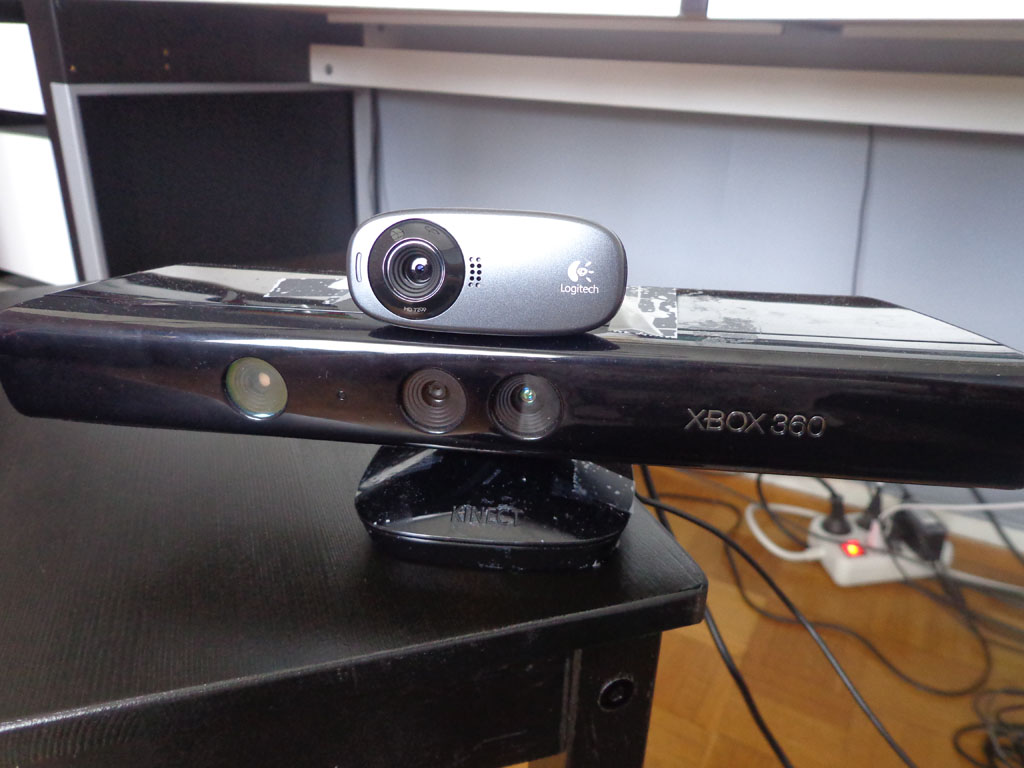
\includegraphics[width=0.7\textwidth]{images/configuration.jpg}
\label{fig:configuration}
\end{figure}


As the reader can guess, projecting a picture at the correct position on a 3D surface is not an easy task and relies on several image processing techniques and linear algebra tools. In order to do so, acquiring the global camera position (of both the Kinect and the webcam) is a necessary task. Indeed, the camera position is important because thanks to it, one can determine the position of a camera (in a given coordinate system) but also the orientation of it. The position and orientation of the cameras are typically given by a translation and rotation matrix (referred as the $\langle R\vert T\rangle$ matrix). Those matrices are involved in the formulas given in ~\ref{sec:Camera pose estimation} (the pinhole camera model formulas) and are used to project a 3D point into its corresponding 2D point, which can be useful to texture the 3D surface with the corresponding IR pictures.\\

Therefore, the focus was first emphasized on finding a suitable library that can give fast and easy camera poses. The following chapters contain a discussion of severals existing tools available on the market.


\section{ARToolKit}
\label{sec:ARToolKit}
The ARToolKit library is a free library that can be used for non-commercial use (GNU general public license) and provides good solutions for augmented reality (AR) applications. As their official website states: "The ARToolKit video tracking libraries calculate the real camera position and orientation relative to physical markers in real time." \cite{artoolkit}. That is, with the help of adequate markers, one can easily determine the pose of a camera in real-time. Figure~\ref{fig:marker} \cite{artoolkit} gives an example of a typical marker used in AR applications.\\


\begin{figure}
\caption{ARToolKit marker}
\centering
    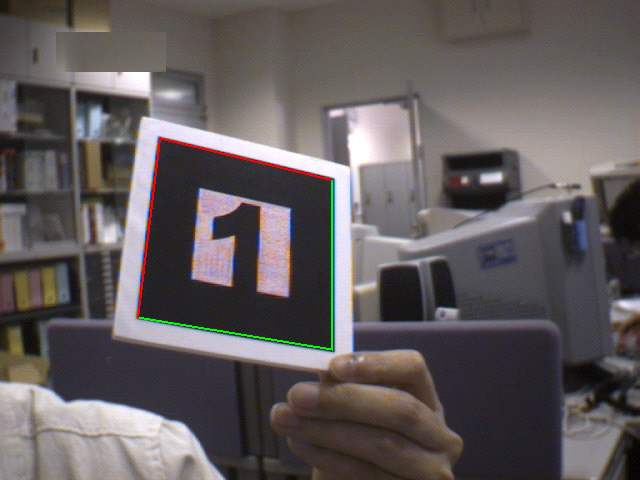
\includegraphics[width=0.7\textwidth]{images/marker.jpg}
\label{fig:marker}
\end{figure}

Markers are often used in computer vision because they present patterns that can be easily recognized by imaging software and therefore their position on the image can be detected with more ease. Of course, one inconvenient is that the markers will have to be physically present on the scene. Also, multiple markers have to be combined together. Indeed, one marker is not enough because lighting condition and/or noise can perturb the detection of it therefore using multiple markers solves this issue but makes the code more complex.\\

At first sight, the ARToolKit library seemed to be a good solution. However, the library has not been updated since 2007, which is a problem since the installation process is not compatible anymore with recent operating systems and hardware. Several installation attempts have been made on different configurations (Windows 7, Ubuntu 12.04 LTS and Mac OSX 10.9 Mountain Lion) but none succeeded.\\


\section{ArUco}
ArUco is a C++ library based on OpenCV. Since OpenCV is used throughout this project, ArUco seemed an interesting alternative to ARToolKit. Like ARToolKit, ArUco uses markers/tags in order to get the camera pose in real time. A great feature of ArUco is that it allows the user to create board of tags. As seen in Figure~\ref{fig:board} \cite{aruco}, a board consists of multiple markers put together.\\

\begin{figure}
\caption{ArUco board}
\centering
    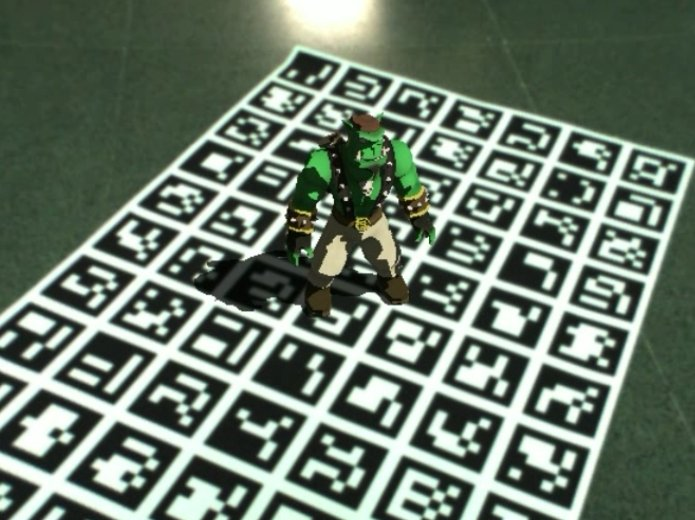
\includegraphics[width=0.7\textwidth]{images/board.jpg}
\label{fig:board}
\end{figure}

Those boards can easily be configured (adjusting the number of horizontal/vertical markers for instance) and their creation is provided by simple scripts from the library.\\

The advantage of using boards over multiple markers is that one can print out the entire board and only one marker from it has to be seen from the camera in order to determine its pose. Also, with multiple markers on a board it is more difficult to lose them all due to lightning conditions or noise. Finally, it provides an easy setup for real world situations. For example, a board (big enough to surround the object of interest) can be printed out and placed on the scene. Then, the ArUco library deals with all the detection and computation steps. Figure~\ref{fig:aruco-demo} \cite{aruco} shows an attempt made where several markers are detected in real-time and the camera pose can be retrieved from it.\\

\begin{figure}[t]
\caption{ArUco demonstration}
\centering
    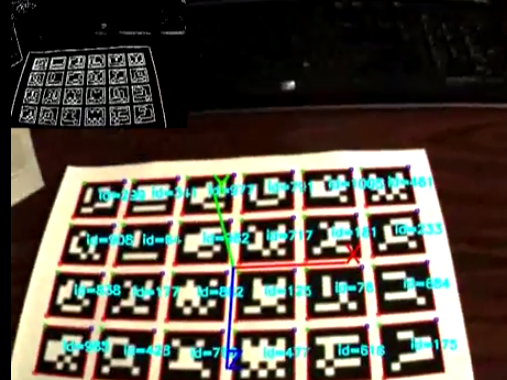
\includegraphics[width=0.7\textwidth]{images/aruco-demo.png}
\label{fig:aruco-demo}
\end{figure}

ArUco has to be installed with cmake, an installation guide is provided on the official website \cite{aruco} and on the sourceforge page \cite{augmented}. 

\section{123D Catch}
123D Catch is an online tool (also available on PC desktop version) developed by Autodesk, it generates a 3D model from 2D pictures. Since only 2D pictures are necessary to obtain a 3D model, 123D Catch seemed to provide easy and simple solutions for the problem. Indeed, if only pictures taken from the external camera are enough to obtain a satisfying 3D model, then this Master Thesis problem would be solved. Therefore, several tests have been conducted in order to determine if 123D Catch can be useful for achieving the desired goal.\\ 

The different tests must reflect real-world situations. For example, a leg, an arm or any other part from a patient's body do not contain a high level of texture details (especially if no body hair are present). Therefore, first a high textured object had been tested, then, tests have been conducted on a less textured object.\\ 

In addition to that, another issues can arise. Indeed, the IR camera will typically produce low resolution pictures with noise on it, which will alter the overall quality of the pictures. In order to get results approaching a real-world situation, two kinds of images have been used:\\

\begin{itemize}
  \item High quality images from a digital camera.
  \item Low resolution grayscale images with noise. 
\end{itemize}


\begin{figure}
\begin{subfigure}{.5\textwidth}
  \centering
  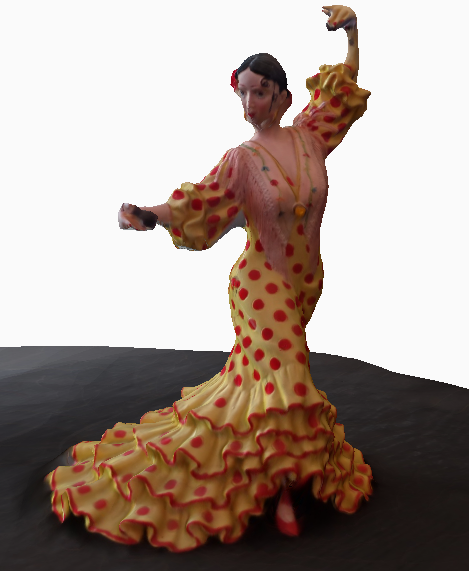
\includegraphics[width=0.8\linewidth]{images/statue-high.png}
  \caption{High resolution}
  \label{fig:statue-high}
\end{subfigure}
\begin{subfigure}{.5\textwidth}
  \centering
  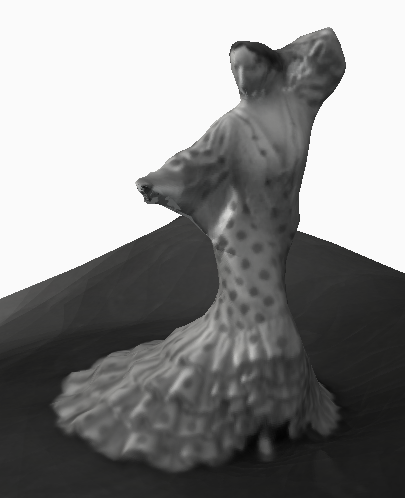
\includegraphics[width=0.8\linewidth]{images/statue-low.png}
  \caption{Low resolution}
  \label{fig:statue-low}
\end{subfigure}
\caption{Statue}
\label{fig:statue}
\end{figure}

\begin{figure}
\begin{subfigure}{.5\textwidth}
  \centering
  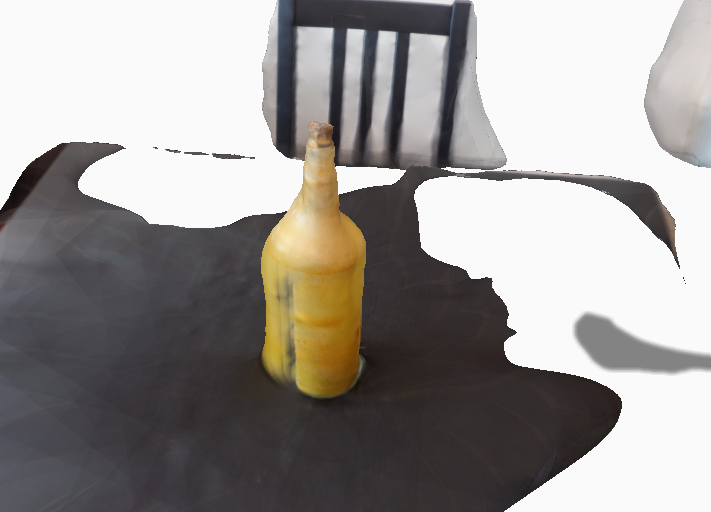
\includegraphics[width=0.95\linewidth]{images/bottle-high.png}
  \caption{High resolution}
  \label{fig:bottle-high}
\end{subfigure}
\begin{subfigure}{.5\textwidth}
  \centering
  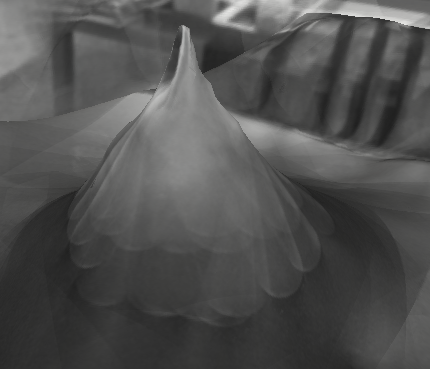
\includegraphics[width=0.8\linewidth]{images/bottle-low.png}
  \caption{Low resolution}
  \label{fig:bottle-low}
\end{subfigure}
\caption{Bottle}
\label{fig:bottle}
\end{figure}

\begin{figure}
\begin{subfigure}{.5\textwidth}
  \centering
  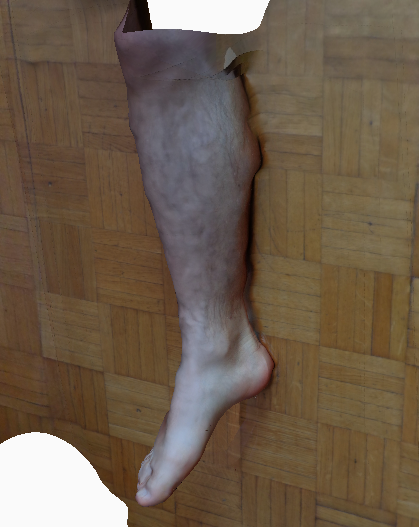
\includegraphics[width=0.8\linewidth]{images/leg-high.png}
  \caption{High resolution}
  \label{fig:leg-high}
\end{subfigure}
\begin{subfigure}{.5\textwidth}
  \centering
  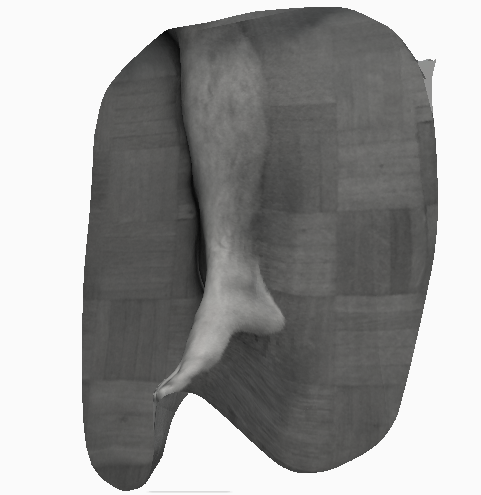
\includegraphics[width=0.8\linewidth]{images/leg-low.png}
  \caption{Low resolution}
  \label{fig:leg-low}
\end{subfigure}
\caption{Leg}
\label{fig:leg}
\end{figure}


At first, tests have been conducted on a highly textured object (a statue), from Figure~\ref{fig:statue} the reader can see that 123DCatch performs well in both a high resolution and low resolution scenarios. \\

On the opposite, Figure~\ref{fig:bottle-high} shows that low textured objects produce poor quality models. Moreover, when low resolution pictures are used (which will be the case in real world scenarios), the results are even worst (see Figure~\ref{fig:bottle-low}) therefore more investigations have been conducted. The Figure~\ref{fig:leg} shows tests conducted on a leg, which represents a good example for the future use of this 3D scan tool. As can be seen from Figure~\ref{fig:leg-high}, high resolution pictures produce good quality model. As for the low resolution version, (Figure~\ref{fig:leg-low}) it seems to not affect much the model.\\

In conclusion, it can be observed than 123D Catch can be a good, cheap and easy solution for our problem.\\

However, a main concern about 123D Catch is that the 3D generation takes a lot of time (usually more than 15 minutes 
depending on the pictures resolution), a Kinect acquisition could provide faster results. Also, as said earlier, some
models do not provided good results therefore some cautions should be raised (it is especially the case when pictures with a level of quality similar of IR images are used). Finally, 123D Catch does not provide any 
API to manipulate nor change the data therefore this solution is neither flexible nor suitable for personal adaptation.

\section{Kinect Fusion}
Kinect Fusion is a project developed by Microsoft researchers. It is a set of libraries being part of the Kinect SDK, it provides solutions for real-time 3D model scanning using the sensors of the Kinect. Several applications samples are provided freely by Microsoft. Those applications are available in C++ and \texttt{C\#} native code.\\ 

One big feature of Kinect Fusion is that only a Kinect is necessary to construct a 3D model of the desired object. There is no need of markers or any other visual information. The scan is done in real-time and several export format exist (\textit{.obj}, \textit{.stl}, \textit{.ply}). \\

However, the reader should be aware that naturally, only windows development is supported. Also, as said in Section~\ref{sec:3D surface reconstruction}, a decent hardware is necessary in order to run the Kinect Fusion Toolkit smoothly. The official website recommends the following minimal configuration \cite{kinect}:


\begin{table}[h]
\caption{Minimal configuration to run Kinect Fusion}
\begin{tabular}{l}
 Desktop PC \\
 Processor 3GHz multi-core\\
 DirectX11 compatible graphics card with 2GB or more of dedicated on-board memory.
\end{tabular}
\label{tab:kinectfusion-minimalconfiguration}
\end{table}

Also, the reader should keep in mind that running Kinect Fusion on a weaker configuration is possible (as long as a DirectX11 compatible graphics card is used). However, it will produce low frame rate and it will make the use of the Kinect Fusion Toolkit tedious (the Kinect camera will have to be maneuvered slowly in order to not lose its camera pose).

As said in~\ref{sec:3D surface reconstruction} the Kinect Fusion Toolkit relies on the iterative closest point (ICP) algorithm. Be it reminded that the ICP algorithm finds the transformation that minimizes the distance between two sets of points. At first, the $\langle R\vert T\rangle$ matrix of the Kinect is set as the identity matrix and then, the ICP algorithm finds the relative transformation between the current frame and the next one and updates this matrix.\\

\section{Discussion}
This section will discuss the implementation choice made. Indeed, each library has advantages and disadvantages. The choice of the good one to use is an important one and would impact a lot the development of this Master Thesis.\\ 

As seen earlier, the ARToolkit library was directly eliminated. At first, this library seemed to provide good solutions for the studied problem. However, due to its old last update date, its installation was considered as hazardous for recent hardware and systems. Also, the lack of support in the long term makes it be an arguable choice.\\

The next library examined was the ArUco library, its development is recent and based on OpenCV. The latter constitutes a solid argument in favor of its use because as it will later be shown, a lot of steps during this Thesis are solved using the OpenCV library. Also, as noticed earlier, the library solves the camera pose problem using boards which constitutes several advantages over single markers.\\

123D Catch seems to offer an easy-to-use solution. However, the results can not always be guaranteed (see Figure~\ref{fig:bottle-low}). Moreover, 123D Catch acts as a \textit{black box} and no API are available to provide further controls or personalizations to the solution.\\

Finally, one last option is the Kinect Fusion Toolkit. The Kinect Fusion Toolkit can provide a simple API to obtain the camera pose in real-time. However, only the Kinect camera pose can be obtained although the set-up requires two cameras (the Kinect and one external camera for IR images acquisition, see Figure~\ref{fig:prototype}). Since the pictures to map on the 3D surface will be taken from the external camera, one needs to find a suitable solution to obtain the pose of the external camera and not only the Kinect.\\

As the reader can see, obtaining the Kinect camera pose is an easy task (thanks to the Kinect Fusion Toolkit). However, obtaining the IR camera pose is more difficult because it often relies on markers (or boards in the case of the ArUco library) placed into the scene. \\

An elegant solution would be to obtain the IR camera pose without relying on external markers. In order to do so, the following idea has been elaborated:\\

The external IR camera needs to be fixed with the Kinect in a way that when the Kinect will move, the external camera will execute the same movement as well. Since the camera moves together, only their relative position is needed.\\ 

Indeed, the relative position will be a $\langle R\vert T\rangle$ matrix, multiplying the matrix describing the Kinect pose by this matrix will give the IR camera pose.\\

The relative position can be computed before running the scan therefore the 3D acquisition is not slowed down. Also, no markers have to be used therefore this solution is the easiest and the most elegant one.\\

An important remark is that at the time of writing this master thesis (Mai 2014), Microsoft is releasing their new Kinect camera for PC. The Kinect v2 provides several improvements over the first version released in 2011. These improvements include:\\

\begin{itemize}
  \item A high-definition color camera able to record in 1080p and capture colors more accurately.
  \item Able to detect heart rate from the facial details of an individual.
  \item An expanded field of view, which allows objects of bigger size and taller people to be closer from the camera.
  \item An improved skeletal tracking. The Kinect sensor can now track six skeletons at the same time. Moreover, the precision has been improved, thumbs and fingers can also be tracked yielding to more accurate skeletal tracking.
  \item Another new feature is what is called the new \textit{active infrared} capability. The new active IR allows the Kinect to capture data even when the light is off and/or the lightning conditions vary. Therefore, the Kinect can run in any lighting conditions making computer-vision-based applications easier to use. 
\end{itemize}


An important point that has not been mentioned yet is that the technology used to acquire live depth map with the Kinect v2 differs from the one present in the first Kinect. Indeed, the first generation of Kinect used a technique called \textit{structured light} (see Section~\ref{sec:3D surface reconstruction}). In the new Kinect, time-of-flight (ToF) technology is used. \\

ToF technology works differently from structured light techniques because in a ToF camera, IR light is emitted then reflected by the objects present in the frame of the camera. The time that the reflected light takes to come back is measured, yielding to the acquisition of the depth information \cite{kolb_time--flight_2010}.\\

The Kinect v2 offers higher accuracy and better tracking capabilities than its predecessor. At this time, Microsoft has not released it yet therefore conducted any test on it is not possible. However, the technology looks promising and further investigations should be made when it will be available for the public.

\section{Solution Description}
As said in Section~\ref{sec:proof of concept - introduction}, a Kinect camera will scan the desired object while an external camera will take pictures which will be then projected on the 3D surface. To project those pictures at the correct locations, one need to performs several steps before. The following subsections describe these steps and give a detailed overview of the solution. 

\subsection{General formula}

The general formula that maps a 3D point to its corresponding 2D point in the pinhole camera model is the following (as a reminder, the reader is invited to consult the Section~\ref{sec:Camera pose estimation}):

\begin{equation}
  q = M\langle R\vert T\rangle Q  
  \label{eq:general equation}    
\end{equation}
\begin{equation}
  q = \begin{bmatrix}
       u \\
       v \\
       w 
     \end{bmatrix}, 
  M = \begin{bmatrix}
       f_x & 0 & c_x \\
       0 & f_y & c_y \\
       0 & 0 & 1
     \end{bmatrix}, 
  \langle R\vert T\rangle =  \begin{bmatrix}
       r_{11} & r_{12} & r_{13} & t_1 \\
       r_{21} & r_{22} & r_{23} & t_2\\
       r_{31} & r_{32} & r_{33} & t_3
     \end{bmatrix},  
  Q = \begin{bmatrix}
       X \\
       Y \\
       Z 
     \end{bmatrix}
\end{equation}

This formula describes the relationship between a 3D point in the real world and its corresponding 2D point inside an image. This information is helpful because the 2D point indicates on which pixels of the picture correspond the 3D point associated with them. If these \textit{(u,v)} coordinates are known, then the color of the associated pixel can be applied on the 3D point, giving a texture mapped on a 3D surface.\\

The following sections will first focus on how the different information constituting the formula can be obtained and then, how to project a simple picture on its corresponding emplacement given a camera pose. Finally, several pictures will be used and results will be given.\\

\subsection{Intrinsic matrix}

The matrix of intrinsic parameters is characterized by the following matrix:

\begin{equation}
  Intrinsics = \begin{bmatrix}
       f_x & s & c_x \\
       0 & f_y & c_y \\
       0 & 0 & 1
     \end{bmatrix}   
\end{equation}

This matrix describes several inner geometric properties of the camera. The following sections will describe each of them. 

\subsubsection{focal length ($f_x$, $f_y$)}
The focal length corresponds to the distance between the pinhole plane and the image plane (see Figure~\ref{fig:pinhole}).\\

In a perfect pinhole camera model, the $f_x$ and $f_y$ are the same for both axis. However, it is often not the case. This can be due to: camera's lens distortions, camera's sensor flaws, error in camera calibration, etc...\\ 

The focal length is measured in pixels.\\

\subsubsection{Principal point offset ($c_x$, $c_y$)}
As seen in Section~\ref{sec:camera calibration} the intersection of the projection center with the image plane is rarely at the exact center of the image plane (see Figure~\ref{fig:principalpoint}) therefore two parameters $c_x$ and $c_y$ are used to adjust this displacement.\\

\begin{figure}
\caption{Principal point offset}
\centering
    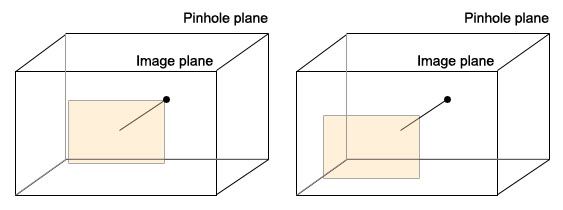
\includegraphics[width=1.0\textwidth]{images/principalpoint.jpg}
\label{fig:principalpoint}
\end{figure}


\subsubsection{Axis skew (s)}
Axis skew causes skew/shear distortions on an object by a specified angle from an axis. See figure~\ref{fig:ulbskew}.


\begin{figure}
\caption{Skew distortion}
\centering
    
\includegraphics[width=1.0\textwidth]{images/ulbskew.jpg}
\label{fig:ulbskew}
\end{figure}

Remark: axis skew s often equals to zero.

\subsubsection{Intrinsic matrix acquisition}
\label{sec:intrinsic acquisition}

The OpenCV library offers several ready-to-use samples and solutions for common imaging problems. Once OpenCV is installed, the samples can be found in the \textit{opencv/samples} folder. For this project, the \textit{calibration} sample located in the C++ folder (\textit{cpp/}) has been used. As said in Section~\ref{sec:camera calibration}, the calibration process relies on a chessboard and several pictures of it to determine the intrinsic matrix.\\

The reader is invited to consult \cite{zhang_flexible_1999} for more details about how OpenCV determines the intrinsic parameters from a chessboard. Also, more information about the acquisition process can be found in section~\ref{sec:Cameras parameters gathering phase}.


\subsection{Extrinsic matrix}

The extrinsic matrix is expressed by the following $\langle R\vert T\rangle$ matrix:

\begin{equation}
\label{eq:extrinsic}
\langle R\vert T\rangle =  \begin{bmatrix}
       r_{11} & r_{12} & r_{13} & t_1 \\
       r_{21} & r_{22} & r_{23} & t_2\\
       r_{31} & r_{32} & r_{33} & t_3
     \end{bmatrix}
\end{equation}  

It represents the orientation and position of the Kinect camera into a given coordinates system. \textit{R} is a rotation matrix describing the Kinect orientation while \textit{T} is a translation vector representing the location of the camera's center inside the coordinates system used.

Obtaining the Kinect camera pose is important for two reasons: 

\begin{itemize}
  \item Testing the formula~\ref{eq:general equation} with only the Kinect in order to verify that the projected texture is valid and hence the formula as well.
  \item As mentioned earlier, an easy approach to obtain the IR camera pose is to first calculate the relative transformation between the IR camera and the Kinect. Once this relative transformation is known, only the Kinect camera pose is needed. 
\end{itemize}

The KinectFusion Toolkit provides straightforward methods to obtain the $\langle R\vert T\rangle$. Moreover, several samples applications are provided by Microsoft offering out of the box 3D surface acquisition tools. More details about this step can be found in Section~\ref{sec:Scanning phase}.

\subsection{Results using only the Kinect}
\label{sec:Results using only the Kinect}

First, in order to prove the validity of the equation~\ref{eq:general equation}, no external cameras are used. Indeed, if good results can already be obtained with pictures taken directly from the Kinect, then it means that both the intrinsic matrix and the $\langle R\vert T\rangle$ matrix acquisition methods are correct therefore the general solution of this master thesis can proceed with pictures taken from an external camera.\\

If the pictures are taken from the Kinect camera, then all the information from the equation~\ref{eq:general equation} can already be found. Indeed, as described in the previous sections, the intrinsic matrix can be obtained via the OpenCV API while the $\langle R\vert T\rangle$ matrix describing the pose of the Kinect camera can easily be obtained with the KinectFusion Toolkit API. Since, in this case, the pictures are taken directly from the Kinect, no further data are required. \\

Figure~\ref{fig:mesh0} shows a mesh obtained through the Kinect Fusion toolkit, Figure~\ref{fig:result from kinect} show this mesh textured with the picture in Figure~\ref{fig:picture from the kinect}. As the reader can see, the projected texture is placed at the correct location thus the data acquired so far are correct. Since the texture mapping is correct, one may wonder why one bothers with the external camera and not just stop here? The problem is, that in real situations, a fluorochrome called indocyanine green (ICG) will be used (recall section~\ref{sec:fluorescence principle}), the ICG emits infrared light after being exited by infrared light from another source. Since the Kinect camera also uses infrared light to obtain depth information \cite{freedman_depth_2008}, some noise/interferences can occur. In one case, the IR light emitted by the external camera could be seen from the Kinect and produce errors. In another case, pictures taken with the external camera could contain the IR dots that the Kinect uses to obtain depth information.  Section~\ref{sec:Hamamatsu camera} discuses about these issues and presents a theoretical study of the Hamamatsu camera (an external camera that can be used to obtain IR information). \\

\begin{figure}
\caption{Mesh of a desk obtained through Kinect Fusion}
\centering
    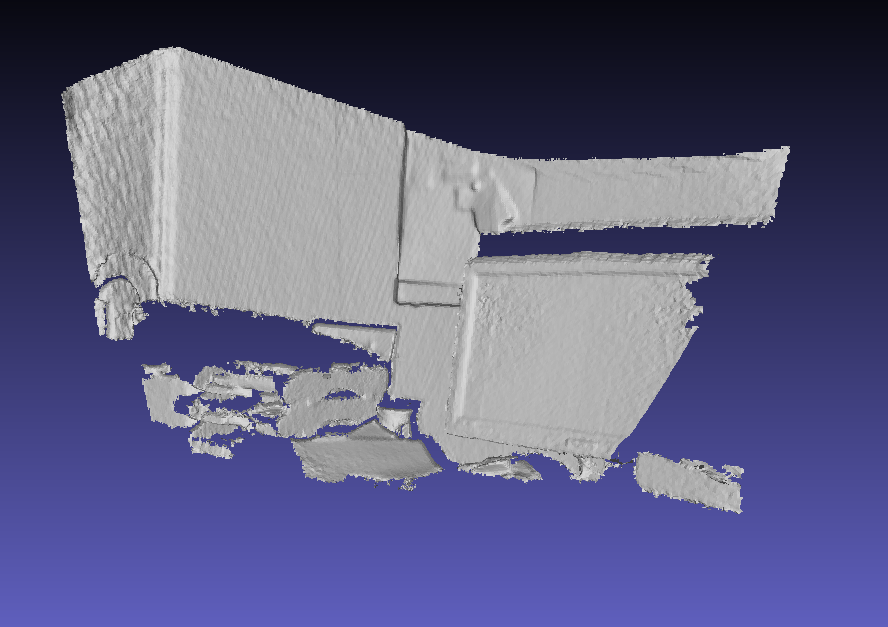
\includegraphics[width=1.0\textwidth]{images/mesh0.png}
\label{fig:mesh0}
\end{figure}

\begin{figure}
\caption{Picture taken from the Kinect camera}
\centering
    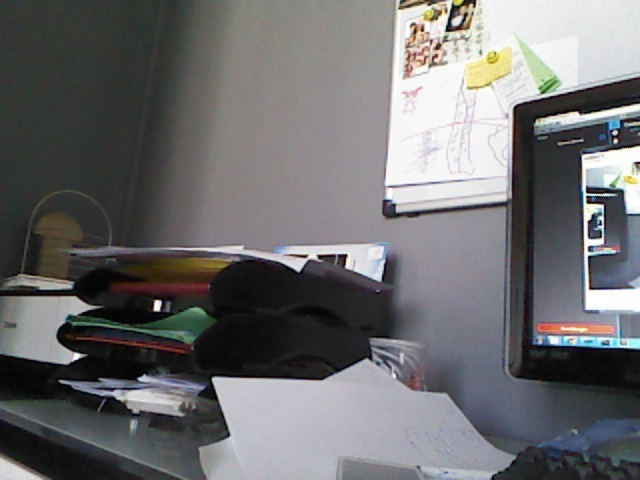
\includegraphics[width=1.0\textwidth]{images/picturefromkinect.jpg}
\label{fig:picture from the kinect}
\end{figure}

\begin{figure}
\caption{Mesh textured with a picture taken from the Kinect camera}
\centering
    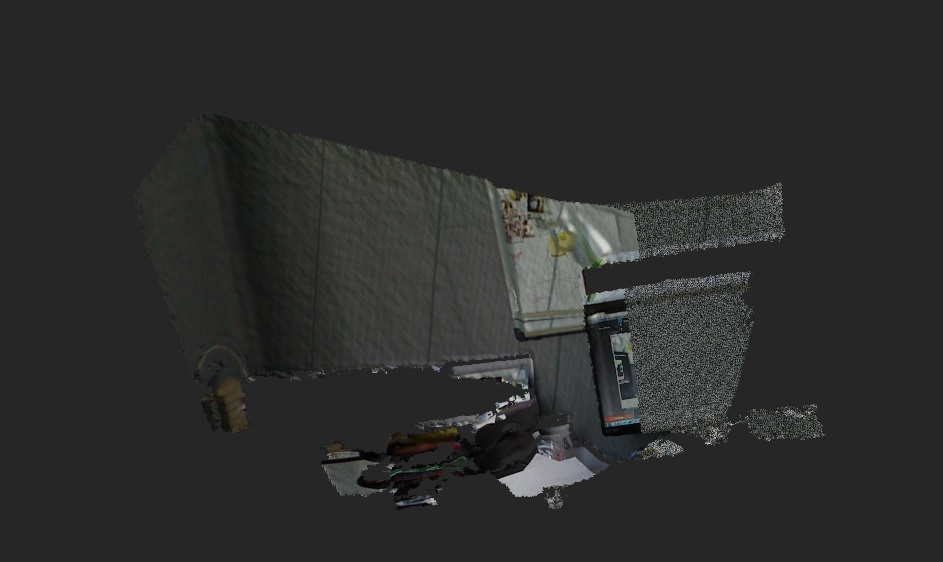
\includegraphics[width=1.0\textwidth]{images/resultfromkinect.jpg}
\label{fig:result from kinect}
\end{figure}


\subsection{External IR camera pose}

As mentioned earlier, an external IR camera will be fixed with the Kinect therefore it is necessary to obtain its extrinsic matrix as well. However, only the extrinsic matrix of the Kinect can be obtained easily (thanks to the KinectFusion Toolkit API). Obtaining the $\langle R\vert T\rangle$ matrix directly from the external camera is not easy and often relies on physical markers present on the scene (see Section~\ref{sec:ARToolKit}). Therefore, a more convenient solution is to use the Kinect $\langle R\vert T\rangle$ matrix obtained through the KinectFusion API and multiply it by a matrix representing the relative transformation between the Kinect and the external camera fixed to it.\\

To do so, one needs to obtain the individual position and rotation of each camera inside a common coordinates system and then simply calculate the difference between them (see Section~\ref{sec:Relative position between the Kinect and the external camera}).


\section{Implementation details}

This master thesis relies on many different libraries and tools. Indeed, as said earlier not only the Kinect Fusion Toolkit is used, but also the OpenCV library. The resolution method consists of combining each of these libraries and tool in an elegant and efficient way. Moreover, often the different steps of the resolution have been written with different languages and API's therefore good communication between them was crucial. Each of these steps was designed for a specific purpose and relies on existing tools and solutions. Developing a good structure and efficient algorithms was important in order to reduce the execution time and provide an easy and automated solution.\\

This section will elaborate what has been discussed before. First, the general structure of the resolution method will be presented. Then, more details will be given for each step of the solution.\\

The general structure and design of the solution is given by Figure~\ref{fig:workflow}. Before capturing and scanning a 3D model, several computations have to be carried out in order to obtain the different cameras information such as the intrinsics and distortion parameters. Only when all the data are gathered, one can start the scanning phase. During the scanning phase several pictures are taken and their corresponding camera positions are registered as well. Finally, the mapping of the pictures on the 3D surface can be operated and the corresponding output files can be viewed by any mesh viewer available on the market (MeshLab was used during this project).\\

\begin{figure}
\caption{General structure of the solution}
\centering
    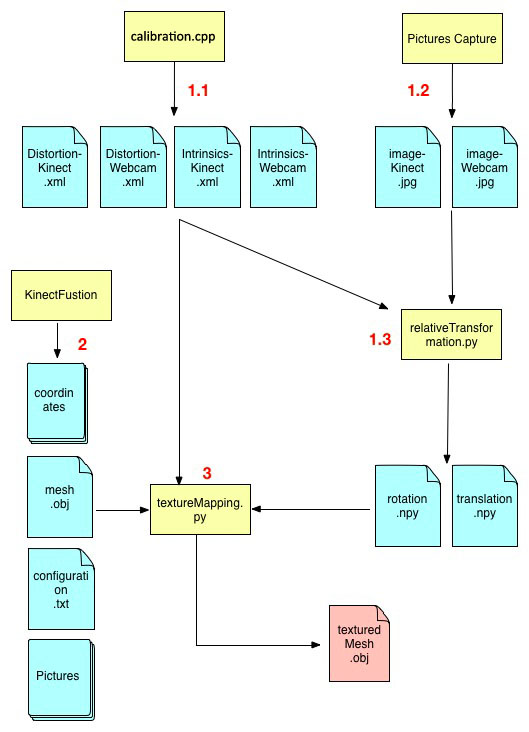
\includegraphics[width=1.0\textwidth]{images/workflow.jpg}
\label{fig:workflow}
\end{figure}

The following subsections will give more details about each phase. Note that all the source code is available on github \cite{github}.

\subsection{Cameras parameters gathering phase}
\label{sec:Cameras parameters gathering phase} 
The first important phase consists of obtaining the different parameters of the cameras (labeled with the number 1 in Figure~\ref{fig:workflow}). As said earlier these parameters are:\\

\begin{itemize}
  \item Intrinsics and distortion parameters.
  \item Relative position between the Kinect and the external camera. 
\end{itemize}

\subsubsection{Intrinsics and distortion parameters}
\label{sec:Intrinsics and distortion parameters}
This section corresponds to the first (1.1) part in Figure~\ref{fig:workflow}.\\

Once OpenCV is installed, the intrinsics and distortion parameters can easily be obtained thanks to the sample program present in the OpenCV installation folder. Since obtaining the intrinsics and distortion parameters is a common task in computer vision, there was absolutely no need to create an application from scratch to do so. Indeed, OpenCV is a reliable library and thanks to its sample programs, this step could be carried out with ease (using the \textit{calibration.cpp} sample).\\ 

The sample program provided by OpenCV requires 25 images in order to output the intrinsic and distortion matrices. Note that this number can be changed in the \textit{default.xml} file together with other information such as the chessboard size and the input file containing the pathname of the different pictures to be used.\\ 

Those pictures represents the chessboard in different position and orientation. For this project, a 6 x 9 chessboard and 25 pictures samples have been used (see Figure~\ref{fig:chessboard} and Figure~\ref{fig:calibration pictures}).\\

\begin{figure}
\caption{Chessboard}
\centering
    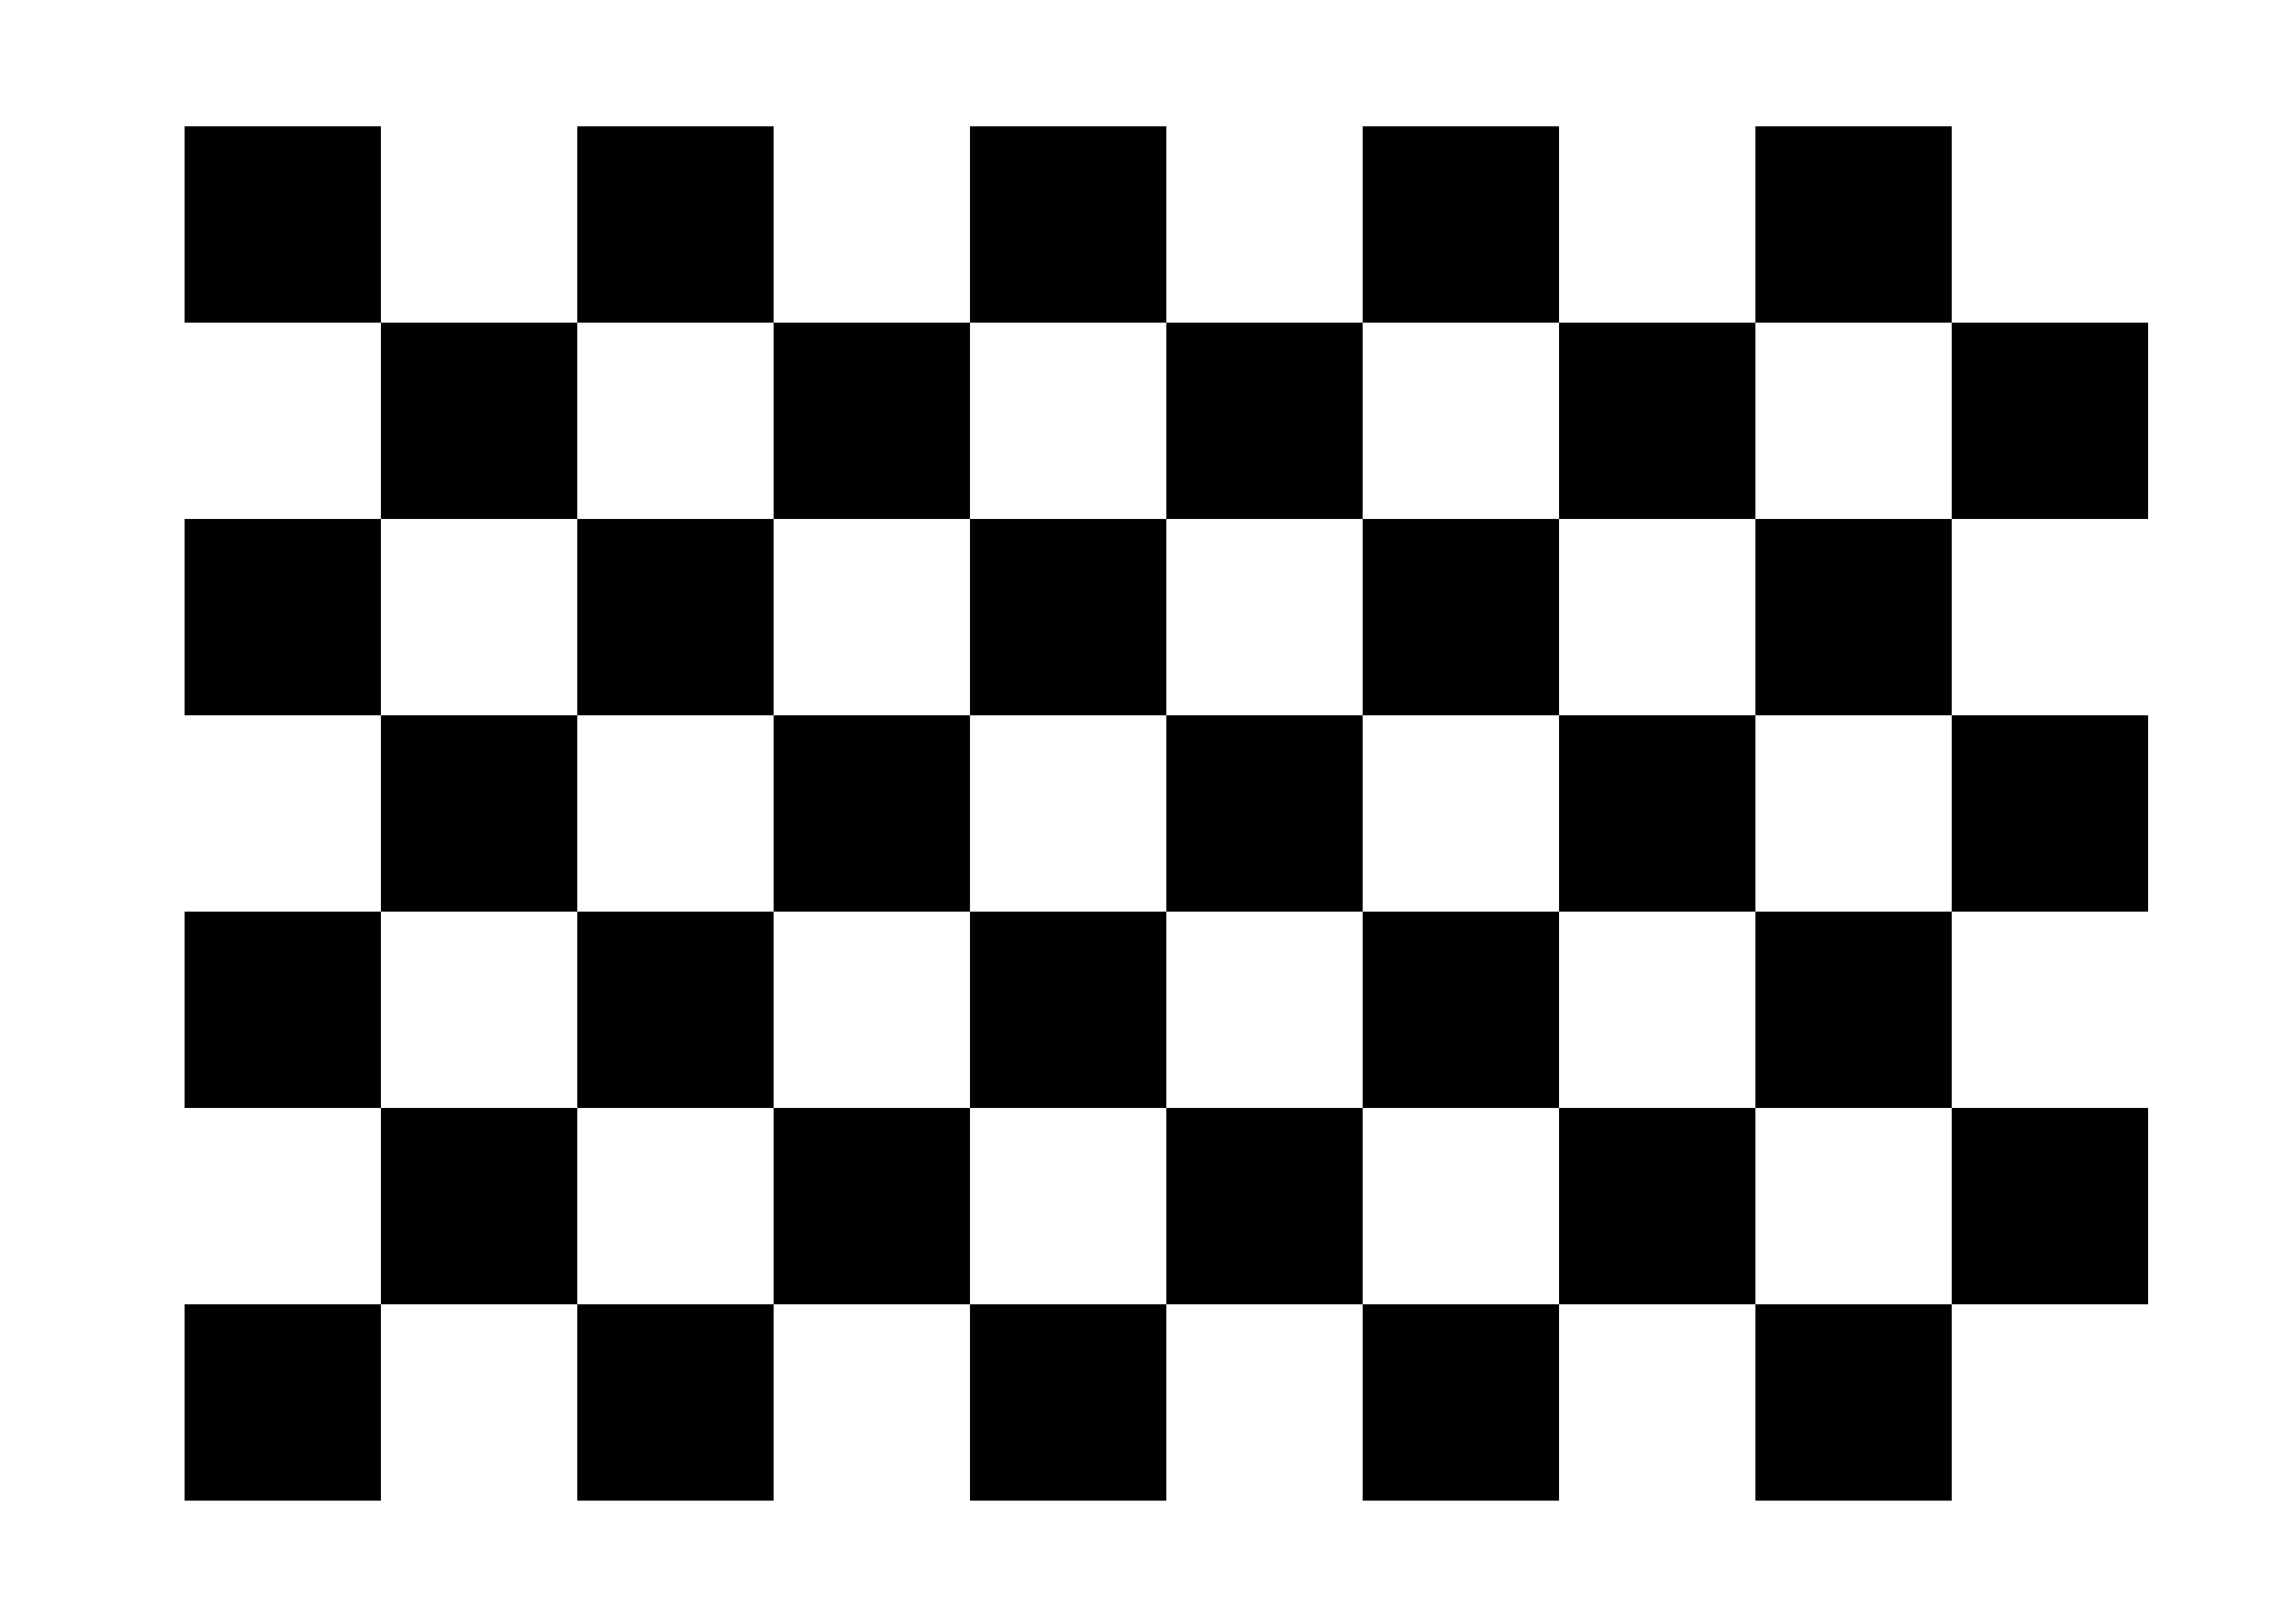
\includegraphics[width=0.5\textwidth]{images/chessboard.png}
\label{fig:chessboard}
\end{figure}

\begin{figure}
\begin{subfigure}{.5\textwidth}
  \centering
  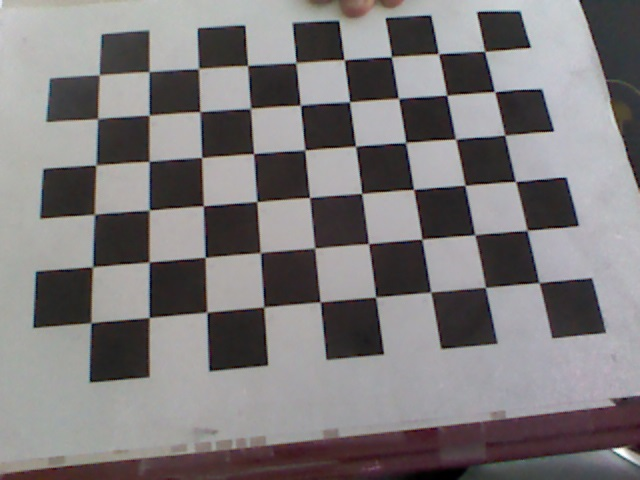
\includegraphics[width=0.8\linewidth]{images/calib1.png}
\end{subfigure}
\begin{subfigure}{.5\textwidth}
  \centering
  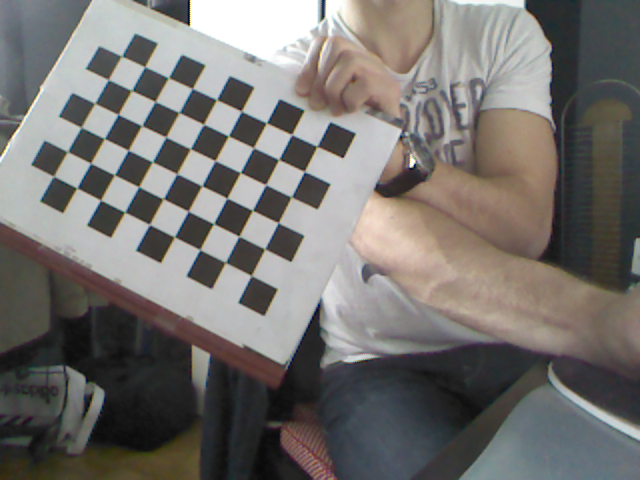
\includegraphics[width=0.8\linewidth]{images/calib2.png}
\end{subfigure}
\begin{subfigure}{.5\textwidth}
  \centering
  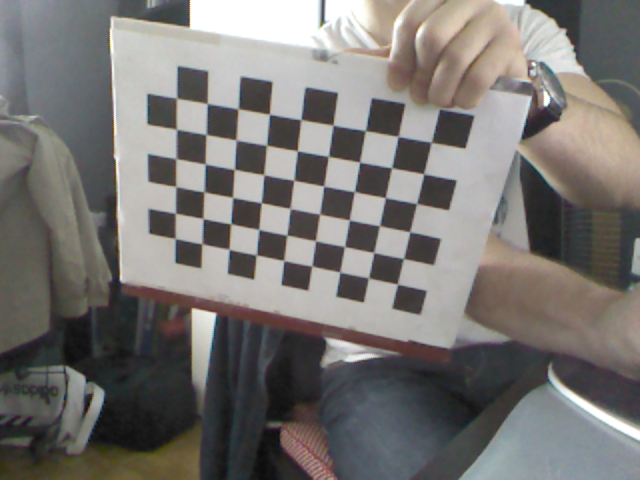
\includegraphics[width=0.8\linewidth]{images/calib3.png}
\end{subfigure}
\begin{subfigure}{.5\textwidth}
  \centering
  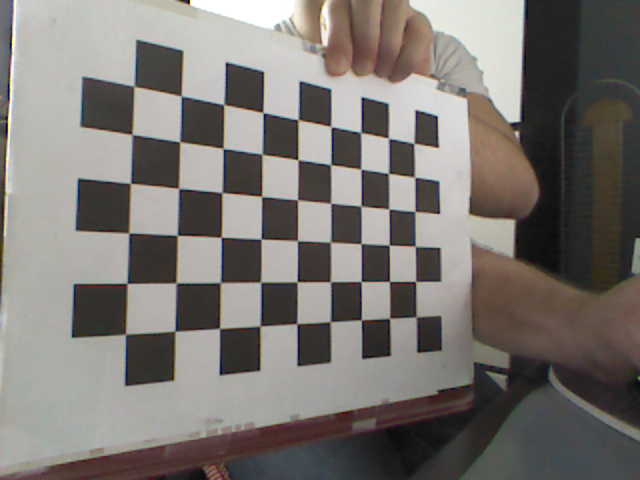
\includegraphics[width=0.8\linewidth]{images/calib4.png}
\end{subfigure}
\caption{Calibration pictures sample}
\label{fig:calibration pictures}
\end{figure}

Another important setting present in the \textit{default.xml} file is the size of the chessboard's squares. Indeed, the calibration process uses no metrics, i.e. one can set the size of the squares in millimeters, meters or any other unit that one finds suitable. After some tests, it has been shown that the Kinect Fusion Toolkit uses meters as unit therefore meters have been used for the calibration step (the chessboard's squares have a 0.024 m size).\\

Once the calibration is done, it outputs the intrinsic matrix but also the distortion matrix in a \textit{.xml} file. However, one important remark is that the sample program provided by OpenCV save the intrinsics and distortion parameters in the same file with other information that are not necessary for this project. Therefore, a slight modification had to be made in order to save only the necessary information in an adequate file structure. As can be seen from Figure~\ref{fig:workflow}, XML files have been used. Indeed, OpenCV can easily store/load matrices and vectors if they are stored in an adequate XML format therefore modifying the original sample program was necessary for the next steps. \\

In addition to that, one should be careful with the orientation of the different pictures used. Indeed, during the tests it has been noticed that the external camera and the kinect camera axis convention is not the same. That is, a picture taken by the Kinect camera will have its x axis flipped if taken by the external camera. This symmetrical difference along the horizontal axis may distort the results therefore before running any computation, one should flip all the pictures along the x axis of one of the two cameras in order to be sure that all the pictures follow the same axis convention.\\

Remark: pictures were captured from the Kinect thanks to the sample \texttt{C\#} \textit{Color Basics} program provided by Microsoft when installing the Kinect SDK. As for the pictures taken from the webcam, a simple OpenCV program was coded. It only consists of displaying the video flow of the camera and taking a picture when the space bar is pressed. The source code of it can be found on Github as well \cite{github}.

After running the calibration program included with OpenCV, the following results have been obtained:\\

\begin{equation}
  Webcam\:intrinsics = \begin{bmatrix}
       828.272 & 0 & 319.5 \\
       0 & 828.272 & 239.5 \\
       0 & 0 & 1
     \end{bmatrix} 
\end{equation}

\begin{equation}
  Kinect\:intrinsics = \begin{bmatrix}
       510.965 & 0 & 319.5 \\
       0 & 510.965 & 239.5 \\
       0 & 0 & 1
     \end{bmatrix} 
\end{equation}

\begin{equation}
  Webcam\:distortion = \begin{bmatrix}
       0.01167 \\
       0.30229  \\
       0 \\
       0 \\
       -2.3152 
     \end{bmatrix} 
\end{equation}

\begin{equation}
  Kinect\:distortion = \begin{bmatrix}
       -0.00471 \\
       0.010791 \\
       0 \\
       0 \\
       -0.17281
     \end{bmatrix} 
\end{equation}

Note that the distortion parameters are used for further steps. Also, the calibration program output an undistorted image at the end of its execution, which is helpful to determine if the calibration step went well and if the parameters are correct. Figure~\ref{fig:calibration result for the kinect} and Figure~\ref{fig:calibration result for the webcam} show the undistorted output images for the webcam and the Kinect respectively.        

\begin{figure}
\caption{Calibration result for the webcam}
\centering
    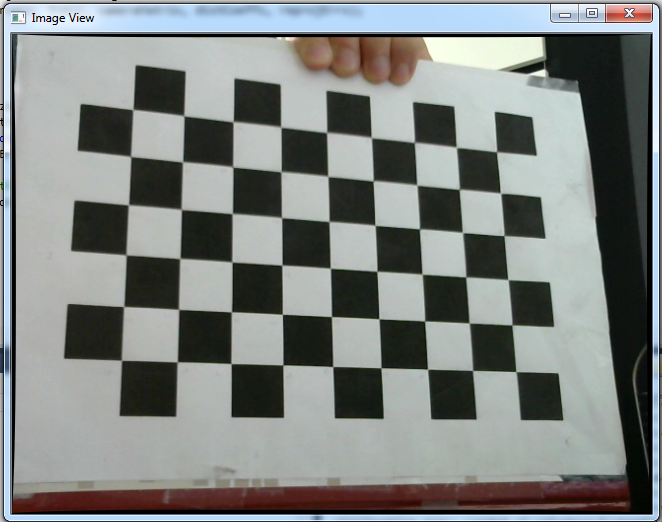
\includegraphics[width=0.7\textwidth]{images/resultCalibWebcam.png}
\label{fig:calibration result for the webcam}
\end{figure}

\begin{figure}
\caption{Calibration result for the Kinect}
\centering
    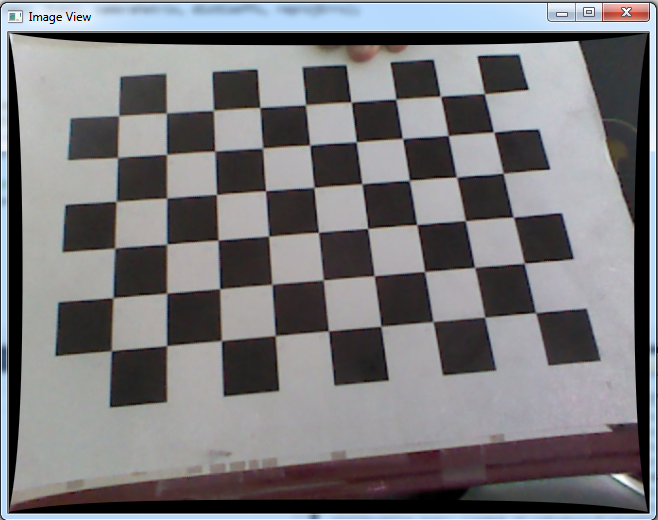
\includegraphics[width=0.7\textwidth]{images/resultCalibKinect.png}
\label{fig:calibration result for the kinect}
\end{figure}

\subsubsection{Relative position between the Kinect and the external camera}
\label{sec:Relative position between the Kinect and the external camera}
This section corresponds to the first (1.2 and 1.3) part in Figure~\ref{fig:workflow}.\\

As said earlier, the main idea to obtain the relative transformation between the Kinect and the external camera is to get the individual pose of each camera. Once these poses are known, determining their relative pose consists of finding the unknown in an equation (see later).\\

To obtain the individual pose of each camera, the \textit{solvePnp()} function of OpenCV is used. This function requires the intrinsics/distortion parameters as well as four images points and their corresponding real-world point. As seen in section~\ref{sec:Intrinsics and distortion parameters}, the intrinsics/distortion matrices can be obtained by using one of the samples provided with the OpenCV library. As for the image/real-world points, one can target the two cameras at the same chessboard and take a picture of it. For each camera, four points of the chessboard have been selected (see Figure~\ref{fig:four points}). The reader can observe the coordinate system used: the origin is at the upper left corner and meters are used again. This configuration is convenient because the same axis convention is used for 2D images by OpenCV.\\

\begin{figure}
\caption{Four points and axis convention}
\centering
    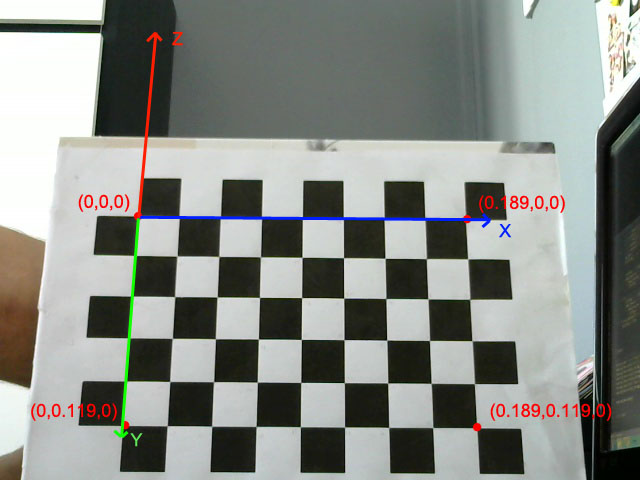
\includegraphics[width=1.0\textwidth]{images/fourPoints.jpg}
\label{fig:four points}
\end{figure}

Now that four real-world points (expressed in meters) are selected, one needs to find their corresponding image coordinates. Once again OpenCV comes in handy because it can easily detect (i.e. find their coordinates in pixels) the inner corners of a chessboard structure using the \textit{findChessboardCorners()} function (see Figure~\ref{fig:inner corners detection}). Since the corners can be detected, the coordinates of the four previous points can be found (expressed in pixels).

\begin{figure}
\caption{Inner corners detection of a chessboard}
\centering
    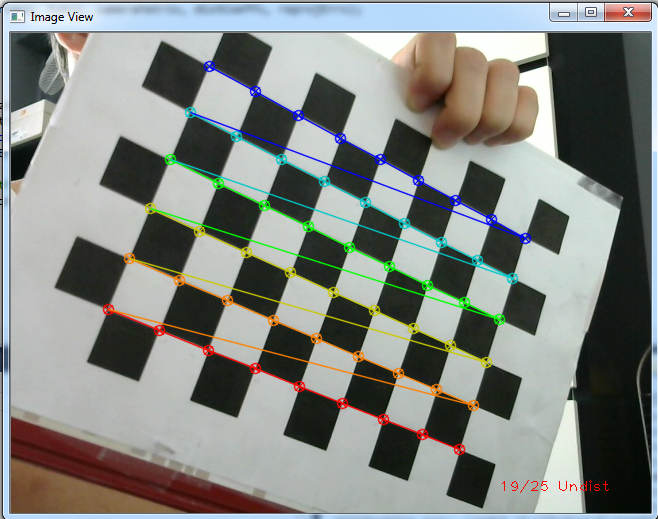
\includegraphics[width=1.0\textwidth]{images/innerCorners.png}
\label{fig:inner corners detection}
\end{figure}


Having now all the required parameters, the \textit{solvePnp()} function can be used. Here is the pseudocode describing all the previous steps. 

\begin{algorithm}[H]
\label{algo:get individual pose}
  \begin{algorithmic}
    \State $intrinsic\gets load(Intrinsics.xml)$
    \State $distortion \gets load(Distortion.xml)$
    \State $imageChessboard \gets  imageRead(image.jpg)$ 

    \State $objPoint1 \gets  (0,0,0)$ 
    \State $objPoint2 \gets  (0.189,0,0)$ 
    \State $objPoint3 \gets  (0,0.119,0)$ 
    \State $objPoint4 \gets  (0.189,0.119,0)$ 
    \State $objPoints \gets  createArray(objPoint1, objPoint2, objPoint3, objPoint4)$ 

    \State $corners \gets  findChessboardCorners(imageChessboard)$
    
    \State $imgPoint1 \gets corners[48]$
    \State $imgPoint2 \gets corners[0]$
    \State $imgPoint3 \gets corners[53]$
    \State $imgPoint4 \gets corners[5]$
    \State $imgPoints \gets  createArray(imgPoint1, imgPoint2, imgPoint3, imgPoint4)$ 

    \State $rvec, tvec \gets  solvePnp(objPoints, imgPoints, intrinsic, distortion)$  
  \caption{Getting the pose of a camera}
  \end{algorithmic}
\end{algorithm}

Note that \textit{corners} is a vector containing all the corners coordinates (expressed in pixels). Therefore, in order to obtain the image points corresponding to the real world corresponding points, one only needs to know how the corners are stored inside the vector and use the appropriate indexes (see Figure~\ref{fig:corners order}). \\

An important remark is that the \textit{solvePnp()} function returns a 3-elements \textit{tvec} (translation) and \textit{rvec} (rotation) vector. Contrary to what one might think, the \textit{tvec} vector does not describe the camera position in the world coordinates system. Indeed, the \textit{tvec} vector is expressed in the camera coordinates system and not in the world coordinates system. In other words, \textit{tvec} is the position of the world origin in camera coordinates. The camera coordinates system always moves with the camera (and the camera is at the origin of it) while the world camera coordinates system is static (with the camera moving within it).\\

This poses a problem since both of the cameras (the Kinect and the webcam) have to be expressed in the same coordinates system in order to find their relative pose. To remedy this issue, the following code is used:\\

\begin{algorithm}[H]
  \begin{algorithmic}
    \State $rvec, tvec\gets solvePnp()$
    \State $rotationMatrix \gets rogrigues(rvec)$
    \State $cameraPosition \gets -rotationMatrix.Transpose() * tvec$ 
  \caption{Converting camera coordinates to world coordinates system}
  \label{algo:pose in world coordinates}
  \end{algorithmic}
\end{algorithm}


This code will transform a camera coordinates system into a world coordinates system allowing the two cameras poses to be expressed inside a common world coordinates system. How does this exactly work ? \\

As a reminder, equation~\ref{eq:extrinsic} represents the camera orientation and location inside the world coordinates system. However, in this case a camera coordinates system is used and not a world coordinates one. The following matrix represents the camera orientation and its location but inside the camera coordinates system (an additional (0,0,0,1) vector has been added to make the matrix square):

\begin{align}
\label{eq:RT camera coordinates system}
\left[
\begin{array}{c|c}
R & T \\
\hline 
0 & 1 \\
\end{array}
\right]
 \end{align}

 The issue is that this matrix represents how the world is transformed relative to the camera coordinates system and not the opposite. Indeed it is fairly more intuitive to have a matrix that represents how the camera is transformed relative to the world coordinates system. Suppose we have a $R_c$ and a $C$ representing respectively the rotation and position of the camera inside a world coordinates system. The inverse of the $\langle R_c\vert C\rangle$ matrix should give the equation~\ref{eq:RT camera coordinates system} (the world-to-camera transformation is simply the inverse of the camera-to-world transformation and vice versa). 

\begin{align}
\label{eq:RT camera and RT world}
\left[
\begin{array}{c|c}
R & T \\
\hline 
0 & 1 \\
\end{array}
\right]
&= 
\left[
\begin{array}{c|c}
R_c & C \\
\hline
0 & 1 \\
\end{array}
\right]^{-1} 
 \end{align} 

The right part of the formula can be decomposed into two matrices describing the rotation and translation.

\begin{align}
    \left [
        \begin{array}{c|c} 
            R_c & C \\
            \hline
            0 & 1 
        \end{array}
    \right ] &= 
    \left [
        \begin{array}{c|c} 
            I & C \\
            \hline
            0 & 1 
        \end{array}
    \right ] 
    \times
    \left [
        \begin{array}{c|c} 
            R_c & 0 \\
            \hline
            0 & 1 
        \end{array}
    \right ] \\
        &=
\left[ \begin{array}{ccc|c} 
1 & 0 & 0 & c_1 \\
0 & 1 & 0 & c_2 \\
0 & 0 & 1 & c_3 \\
  \hline
0 & 0 & 0 & 1
\end{array} \right] \times
\left[ \begin{array}{ccc|c} 
r_{1,1} & r_{1,2} & r_{1,3} & 0  \\
r_{2,1} & r_{2,2} & r_{2,3} & 0 \\
r_{3,1} & r_{3,2} & r_{3,3} & 0 \\
  \hline
0 & 0 & 0 & 1
\end{array} \right] 
\end{align}

Distributing the inverse on these two matrices gives the following result (note that $(AB)^{-1} = B^{-1}A^{-1}$):

\begin{align}
\left[
\left[
  \begin{array}{c|c}
    I & C \\
    \hline
    0 & 1 \\
  \end{array}
\right]
\left[
  \begin{array}{c|c}
    R_c & 0 \\
    \hline
    0 & 1 \\
  \end{array}
\right]
\right]^{-1} 
&= 
\left[
\begin{array}{c|c}
R_c & 0 \\
\hline
0 & 1 \\
\end{array}
\right]^{-1} 
\left[
\begin{array}{c|c}
I & C \\
\hline
0 & 1 \\
\end{array}
\right]^{-1} 
\end{align} 

Finally, applying the inverse and the multiplication gives:

\begin{align}
\left[
  \begin{array}{c|c}
    R_c & 0 \\
    \hline
    0 & 1 \\
  \end{array}
\right]^{-1} 
\left[
  \begin{array}{c|c}
    I & C \\
    \hline
    0 & 1 \\
  \end{array}
\right]^{-1} 
&= 
\left[
\begin{array}{c|c}
R_c^T & 0 \\
\hline
\boldsymbol{0} & 1 \\
\end{array}
\right]
\left[
\begin{array}{c|c}
I & -C \\
\hline
\boldsymbol{0} & 1 \\
\end{array}
\right] \\
&= 
\left[
\begin{array}{c|c}
R_c^T & -R_c^TC \\
\hline
\boldsymbol{0} & 1 \\
\end{array}
\right] 
\end{align} 

This results comes from the fact that the inverse of a rotation matrix is its transpose while the inverse of a translation vector is simply its negation. Here is a recap of the full development (note that the explanations and formulas were taken from \cite{dissecting}): 

\begin{align}
\left[
\begin{array}{c|c}
R & \boldsymbol{T} \\
\hline 
\boldsymbol{0} & 1 \\
\end{array}
\right]
  &= 
\left[
\begin{array}{c|c}
R_c & C \\
\hline
\boldsymbol{0} & 1 \\
\end{array}
\right]^{-1} \\
  &= 
\left[
\left[
\begin{array}{c|c}
I & C \\
\hline
\boldsymbol{0} & 1 \\
\end{array}
\right]
\left[
\begin{array}{c|c}
R_c & 0 \\
\hline
\boldsymbol{0} & 1 \\
\end{array}
\right]
\right]^{-1} & \text{(decomposing rigid transform)} \\
&= 
\left[
\begin{array}{c|c}
R_c & 0 \\
\hline
\boldsymbol{0} & 1 \\
\end{array}
\right]^{-1} 
\left[
\begin{array}{c|c}
I & C \\
\hline
\boldsymbol{0} & 1 \\
\end{array}
\right]^{-1} & \text{(distributing the inverse)}\\
&= 
\left[
\begin{array}{c|c}
R_c^T & 0 \\
\hline
\boldsymbol{0} & 1 \\
\end{array}
\right]
\left[
\begin{array}{c|c}
I & -C \\
\hline
\boldsymbol{0} & 1 \\
\end{array}
\right] & \text{(applying the inverse)}\\
&= 
\left[
\begin{array}{c|c}
R_c^T & -R_c^TC \\
\hline
\boldsymbol{0} & 1 \\
\end{array}
\right] & \text{(matrix multiplication)}
\end{align} 

The reader can see that the relationship between the camera coordinates and the world coordinates can be expressed by the following formulas:

\begin{align}
R  &= R_c^T \\
T &= -RC 
\end{align}

Therefore the position of the camera inside the world can be given by:

\begin{align}
C &= -R^{-1}T\\
  &= -R^TT 
\end{align}

Which is why the algorithm~\ref{algo:pose in world coordinates} uses the same development in order to get the positions of the two cameras inside the same world coordinates system. \\

As for \textit{rvec}, it is a 3-elements rotation vector, the \textit{rodrigues()} method transforms this rotation vector into a 3x3 rotation matrix. Note that rotation vectors define a more compact way to represent a rotation matrix. As an example, a rotation of $\pi/2$ radiants around the x axis would be represented by the following vector:

\begin{equation}
\begin{bmatrix} 
\pi/2 & 0 & 0 
\end{bmatrix}
\end{equation}


Sometimes it is more convenient to represent a rotation with a vector in order to simplify further computations. Indeed, once the rotation and translation vectors are obtained for both the Kinect and the external camera, getting their relative transformation is straightforward:

\begin{algorithm}[H]
  \begin{algorithmic}
    \State $R \gets rotationCamera - rotationKinect$
    \State $R \gets rogrigues(R)$
    \State $T \gets positionCamera - positionKinect$ 
  \caption{Getting the transformation between the Kinect and the webcam}
  \end{algorithmic}
\end{algorithm}

The reader can notice that in this case, using rotation vectors instead of rotation matrices was more convenient since it facilitates the acquisition of the rotation matrix between the Kinect and the external camera.\\

Now that the relative transformation is obtained, one needs only to multiply the $\langle R\vert T\rangle$ matrix from~\ref{eq:general equation} with the $\langle R\vert T\rangle$ matrix representing the relative transformation between the Kinect and the webcam.\\

In order to do so, homogeneous coordinates are used. Homogeneous coordinates consists of adding a fourth row to the $\langle R\vert T\rangle$ matrices in order to transform them in square matrices, which is necessary for the matrix multiplication (see equation~\ref{eq: RT homogeneous}).

\begin{equation}
\label{eq: RT homogeneous}
  \langle R\vert T\rangle =  \begin{bmatrix}
       r_{11} & r_{12} & r_{13} & t_1 \\
       r_{21} & r_{22} & r_{23} & t_2 \\
       r_{31} & r_{32} & r_{33} & t_3 \\
       0 & 0 & 0 & 1
     \end{bmatrix}
\end{equation}

\begin{figure}[H]
\caption{Corners order}
\centering
    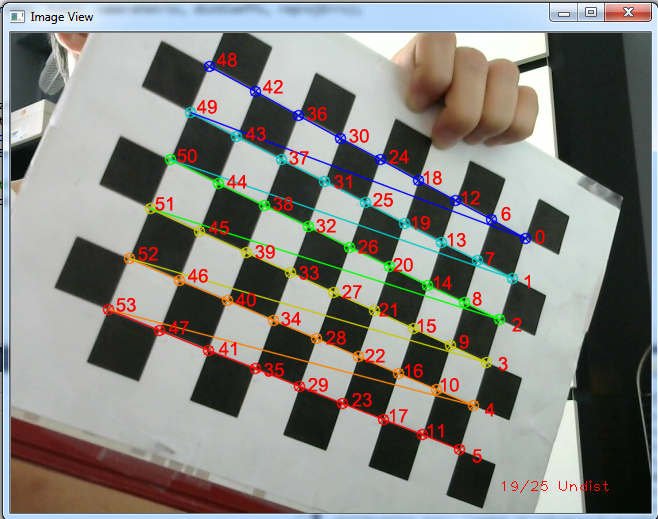
\includegraphics[width=1.0\textwidth]{images/cornersOrder.png}
\label{fig:corners order}
\end{figure}

\subsection{Scanning phase} 
\label{sec:Scanning phase}
This section corresponds to second part in Figure~\ref{fig:workflow}.\\

Once the Kinect development tools are installed, one can find several sample programs in the installation folder. One of them is the \textit{KinectFusionExplorer - WPF} application. It consists of an easy and user friendly application made by Microsoft to perform 3D surface acquisition (see Figure~\ref{fig:Kinect Fusion Toolkit}).\\ 

\begin{figure}
\caption{Kinect Fusion Toolkit}
\centering
    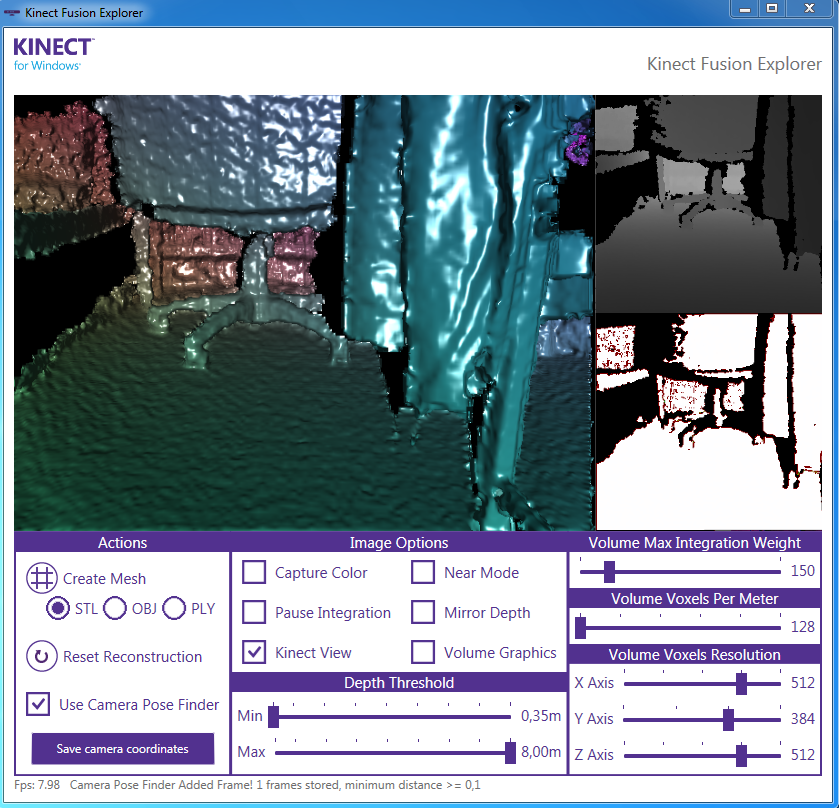
\includegraphics[width=1.0\textwidth]{images/kinectApplication.png}
\label{fig:Kinect Fusion Toolkit}
\end{figure}

This sample application also provides a way to save the 3D surface obtained into a \textit{.obj/.ply/.stl} file. For this project the \textit{.obj} file has been chosen because its structure is easy to modify and to associate with an \textit{.mtl} file (the file responsible for texture mapping).\\

Concerning the Kinect extrinsic matrix, it can easily be obtained by using the provided API from Microsoft (the method \textit{worldToCameraTransform()} returns it). For this project, the sample \textit{KinectFusionExplorer - WPF} application has been modified, a button \textit{save camera coordinates} has been added in the user interface allowing the user to save the Kinect camera pose in an external file when it is necessary (see Figure~\ref{fig:Kinect Fusion Toolkit}). The modified program will produce \textit{coordinates.txt} files and a \textit{configuration.txt} file as well, which indicates the number of coordinates taken during the 3D surface acquisition phase.\\

An important remark is that each time the \textit{save camera coordinates} button is pressed, the user also needs to take a picture with the external camera. A separate OpenCV program \textit{DisplayCamera.py} has been created for that purpose.\\

Once the scanning is over, the 3D surface can be saved by using the adequate file format (\textit{.obj}). Figure~\ref{fig:workflow} shows a recap of the different files produced during this step.

\subsection{Texture mapping phase} 
\label{sec:Texture mapping phase}
Now that the intrinsic parameters, the Kinect extrinsic matrix and the relative transformation between the cameras are known, the final step of the resolution can begin.

The general Equation~\ref{eq:general equation} outlines the different steps needed to map a 3D point into its corresponding 2D point. Once the corresponding 2D point is known, its 2D coordinates indicates which pixel will be used inside the adequate picture in order to texture the 3D surface. Figure~\ref{fig:Texture mapping description} illustrates this and as the reader might notice, one information is still missing. Indeed, the $\left[ \begin{smallmatrix} X & Y & Z \end{smallmatrix} \right]$ vector still needs to be obtained.\\

\begin{figure}
\caption{Texture mapping description}
\centering
    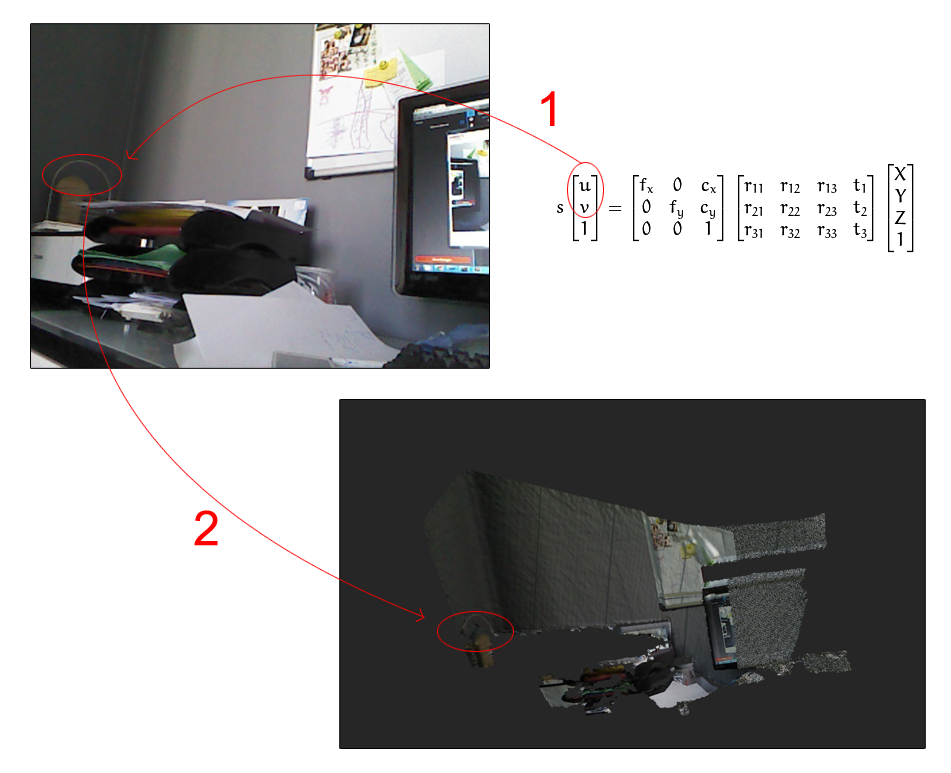
\includegraphics[width=1.0\textwidth]{images/mappingDescription.png}
\label{fig:Texture mapping description}
\end{figure}

This vector corresponds to the coordinates of a point of the 3D surface. Recall that those coordinates are given by the \textit{.obj} file acquired during the previous step. An \textit{.obj} file has the following structure (lines starting with \# are comments):\\

\noindent\#List of vertices\\ 
v 0.538 0.207 -0.361\\
v 0.535 0.207 -0.353\\
v 0.538 0.214 -0.361\\
...\\

\noindent\#List of texture coordinates (see later)\\
vt 0.0 0.0\\
vt 0.0 0.5\\
vt 0.5 0.0\\
...\\

\noindent\#List of normals\\
vn 0.375 -0.366 0.850\\
vn 0.240 -0.259 0.935\\
vn 0.217 -0.119 0.968\\
...

\noindent\#List of faces\\
f 1//1 2//2 3//3\\
f 4//4 5//5 6//6\\
f 7//7 8//8 9//9\\
...\\

A 3D mesh is often formed by triangles, each corner of the triangle is a vertex. The \textit{.obj} file lists the coordinates of all the vertices and normals but it also contains a list of faces definitions. A face is defined by its vertices, normals and texture coordinates (see later). Each corner of a face is defined by the following:\\

\noindent f Vertex index/Texture coordinates index/Normal index \\

Therefore, the following examples defines a triangle by using the first,second and third vertex/normal listed in the \textit{.obj} file:\\

\noindent f 1//1 2//2 3//3\\

Such definition does not take into account the texture associated with the face. Indeed, a \textit{.obj} file of a textured mesh needs to contain texture coordinates inside it. Each mesh can contain several texture materials associated with it. A picture can be a texture material, if it is the case, the texture coordinates inside the \textit{.obj} file indicate the coordinates of specific pixels inside the picture: \\

\noindent vt u v\\

Where \textit{u} and \textit{v} are normalized (their value is between 0 and 1) and describe image coordinates of a texture (see Figure~\ref{fig:Texture mapping description} and Figure~\ref{fig:Texture mapping example} \cite{blogtartiflop}). When using textures, a \textit{.mtl} file needs to be associated with the \textit{.obj} file. A \textit{.mtl} file contains material information, each material can be specified by its color, texture, illumination, etc. \textit{.mtl} files are convenient since multiple materials can be defined inside the same file therefore all the pictures taken by the external camera can be regrouped in a single \textit{.mtl} file:\\

\noindent newmtl texture0\\
  Ns 10.0000\\
  Ni 1.5000\\
  ...\\
  illum 2\\
  Ka 0.0000 0.0000 0.0000\\
  Kd 0.5880 0.5880 0.5880\\
  ...\\
  map\_Ka Images/image0.jpg\\
  map\_Kd Images/image0.jpg\\

\noindent newmtl texture1\\
  Ns 10.0000\\
  Ni 1.5000\\
  ...\\
  illum 2\\
  Ka 0.0000 0.0000 0.0000\\
  Kd 0.5880 0.5880 0.5880\\
  ...\\
  map\_Ka Images/image1.jpg\\
  map\_Kd Images/image1.jpg \\ 

\begin{figure}
\caption{Texture mapping example}
\centering
    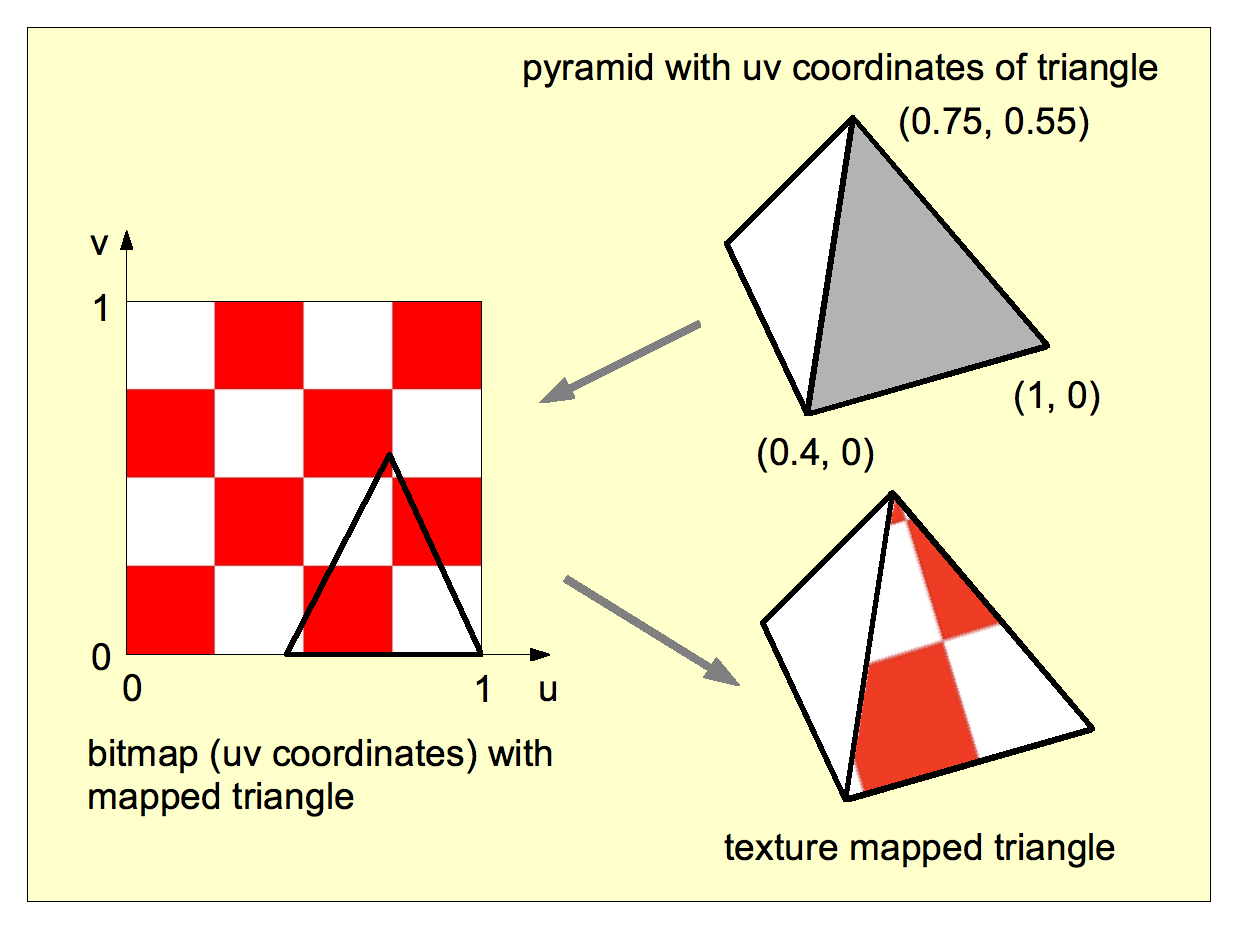
\includegraphics[width=1.0\textwidth]{images/textureMappingExample.png}
\label{fig:Texture mapping example}
\end{figure}


The following paragraphs will outline the general solution found to produce these texture coordinates and effectuate the texture mapping.\\

The \textit{.obj} files produced by the Kinect are usually big (more than 100Mb) therefore before starting any computation one important step is to preprocess the entire file and put its data inside lists since a disk access is usually slower than a direct memory access. Therefore, the first step is to create lists containing the vertices and normals coordinates. Note that after running some tests it has been estimated that preprocessing the entire file reduces 50\% of the execution time.\\ 

Another optimization is to use the Numpy library. The Numpy library is a python library used for scientific computing, it provides several tools for linear algebra and matrix manipulation therefore its utilization facilitated many steps  during the resolution of this master thesis.\\

The next step consists of applying the formula~\ref{eq:general equation} on each vertex coordinates. If the results are inside the pictures frame (for example, if the pictures have a 640 x 480 size then the coordinates \textit{(u,v)} must be inside these dimensions), then the results are kept and a new texture coordinates is created. If the results are not inside the pictures frame, then they are discarded. The algorithm runs on all the vertices coordinates and create the texture coordinates associated with them one after the other.


\begin{algorithm}[H]
  \begin{algorithmic}
    \State $intrinsics \gets loadIntrinsics()$ 
    \State $vertices\_list, normals\_list \gets preprocessFile()$ 
    \For{picture i}
      \State $\langle R\vert T\rangle \gets getRT(i)$ 
      \For{vertex coordinates j}
        \State $\left[ \begin{smallmatrix} X & Y & Z \end{smallmatrix} \right] \gets vertices\_list.getCoordinates(j)$ 
        \State $\left[ \begin{smallmatrix} U & V & W \end{smallmatrix} \right] \gets intrinsics * \langle R\vert T\rangle * \left[ \begin{smallmatrix} X & Y & Z \end{smallmatrix} \right] $ 
        \State $\left[ \begin{smallmatrix} U & V & 1 \end{smallmatrix} \right] \gets normalizeUV(\left[ \begin{smallmatrix} U & V & W \end{smallmatrix} \right])$
        \If{u and v inside picture i dimension} 
          \State $uv\_texture\_coordinates\_list.append(vt  + u  + v)$
          \State $faces \gets createTexturedFace()$ 
          \If{\textit{faces} contains 3 faces} 
            \State $faces\_list[i].append(faces)$
            \State $faces.reinit()$
          \EndIf
        \Else 
          \State $faces \gets createUntexturedFace()$
          \If{\textit{faces} contains 3 faces} 
            \State $untextured\_faces\_list.append(faces)$
            \State $faces.reinit()$
          \EndIf
        \EndIf
      \EndFor   
    \EndFor 
  \caption{Texture mapping algorithm}
  \label{algo:Texture mapping algorithm}
  \end{algorithmic}
\end{algorithm}

Algorithm~\ref{algo:Texture mapping algorithm} shows the main steps of the texture mapping process. One important remark is how the different faces are defined. Indeed, recall that the \textit{.obj} file structure defines two ways to declare faces. One with the texture information and one without it. The program maintains several indexes indicating: the current vertex being treated, its corresponding normal coordinates and the current texture coordinates created. When the \textit{(u,v)} coordinates are inside the picture frame, a face is defined like this:\\

\noindent Vertex index/Texture coordinates index/Normal index \\

When the \textit{(u,v)} coordinates are not inside the picture frame, a face without texture is created simply like this:\\

\noindent Vertex index//Normal index \\

Therefore, the \textit{createTexturedFace()} and \textit{createUntexturedFace()} procedures create several faces and when three of them are created in a row, they are put inside some lists containing all faces definitions to write in the final textured \textit{.obj} file.\\  

Finally, at the end of the execution after that all the pictures were treated, the different lists contain all the information needed to define a textured \textit{.obj} file, i.e. the vertices coordinates, the normals coordinates, the texture coordinates and the different faces definitions (the ones with textures associated with them and the ones without). The watchful reader can notice that the \textit{faces\_list[i].append(faces)} instruction gathers the faces belonging to the same picture since one needs to specify which material to use for each picture (see Figure~\ref{fig:multipleTextureOBJFile}). Also, Figure~\ref{fig:multipleTextureOBJFile} gives an overall view of the resulting textured \textit{.obj} file.

\begin{figure}
\caption{Multiple textures inside a .obj file}
\centering
    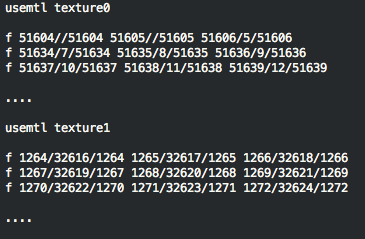
\includegraphics[width=1.0\textwidth]{images/multipleTextureOBJFile.png}
\label{fig:multipleTextureOBJFile}
\end{figure}

\section{Results}
\label{sec:Results}

The previous sections described in details the implementation of the solution, this section will describe and discuss the results obtained with the final application.\\

As a reminder, Figure~\ref{fig:workflow} shows the work flow and the different steps needed to obtain a textured 3D surface. In opposition with the results showed in Section~\ref{sec:Results using only the Kinect}, where only pictures taken directly from the Kinect where projected on the 3D surface, this section describes the different results obtained through the external camera. During the scanning phase, several pictures where taken with a webcam and its corresponding positions were also acquired thanks to the modified KinectFusionExplorer application (see Section~\ref{sec:Scanning phase}). Figure~\ref{fig:result1}, Figure~\ref{fig:result2}, Figure~\ref{fig:result3} and Figure~\ref{fig:result4} show the different results obtained, as the reader can notice some projection errors can be observed at some parts on the scene. Indeed, this is due because the camera acquiring the 3D surface is not aligned with the one taking the pictures. That is, the cameras do not target the same area therefore the texture mapping can not be operated accurately everywhere. This phenomenon is called the \textit{parallax problem} and often takes place in cameras where the viewfinder is located above the lens taking the picture. One way to reduce the \textit{parallax problem} would be to use wide angle lens but unfortunately the current infrared cameras do not have this advantage.

\begin{figure}
\caption{Result 1}
\centering
    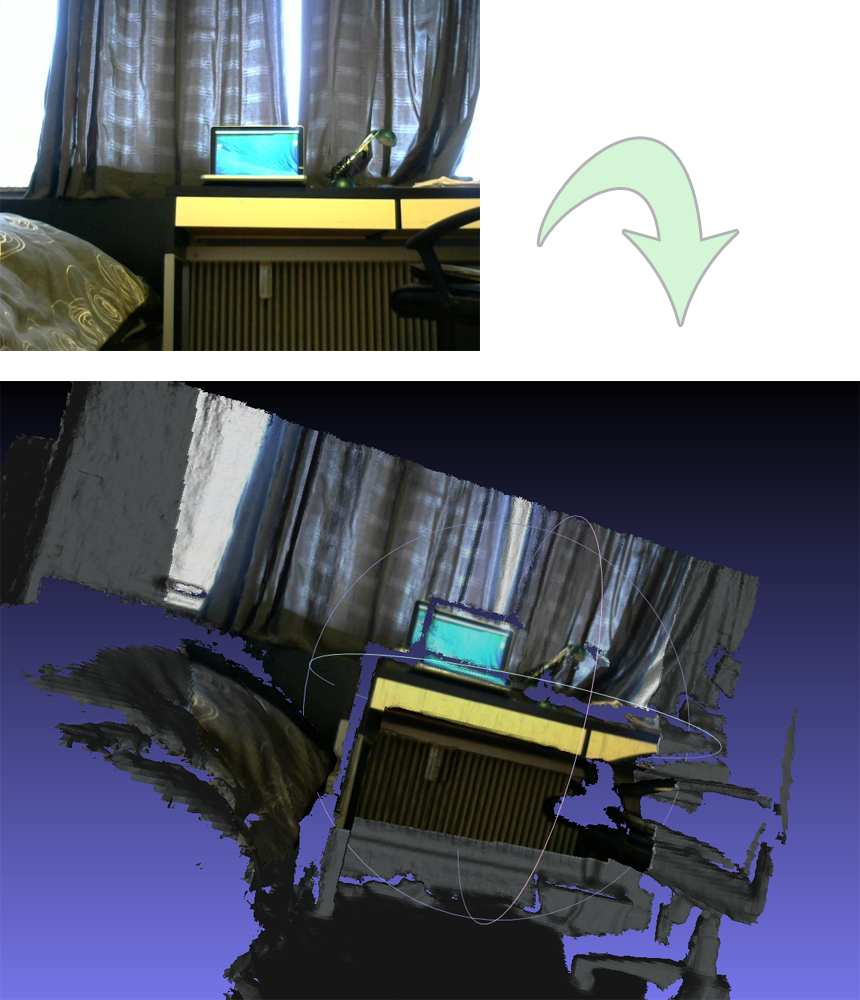
\includegraphics[width=1.0\textwidth]{images/result1.png}
\label{fig:result1}
\end{figure}

\begin{figure}
\caption{Result 2}
\centering
    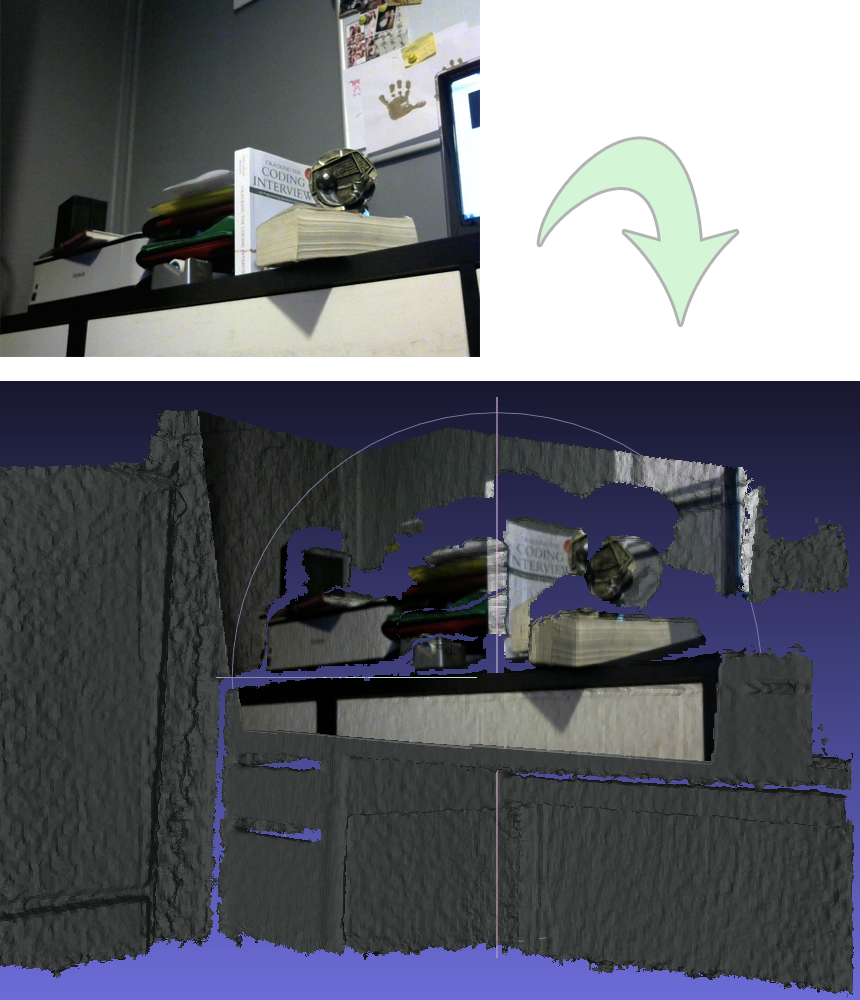
\includegraphics[width=1.0\textwidth]{images/result2.png}
\label{fig:result2}
\end{figure}

\begin{figure}
\caption{Result 3}
\centering
    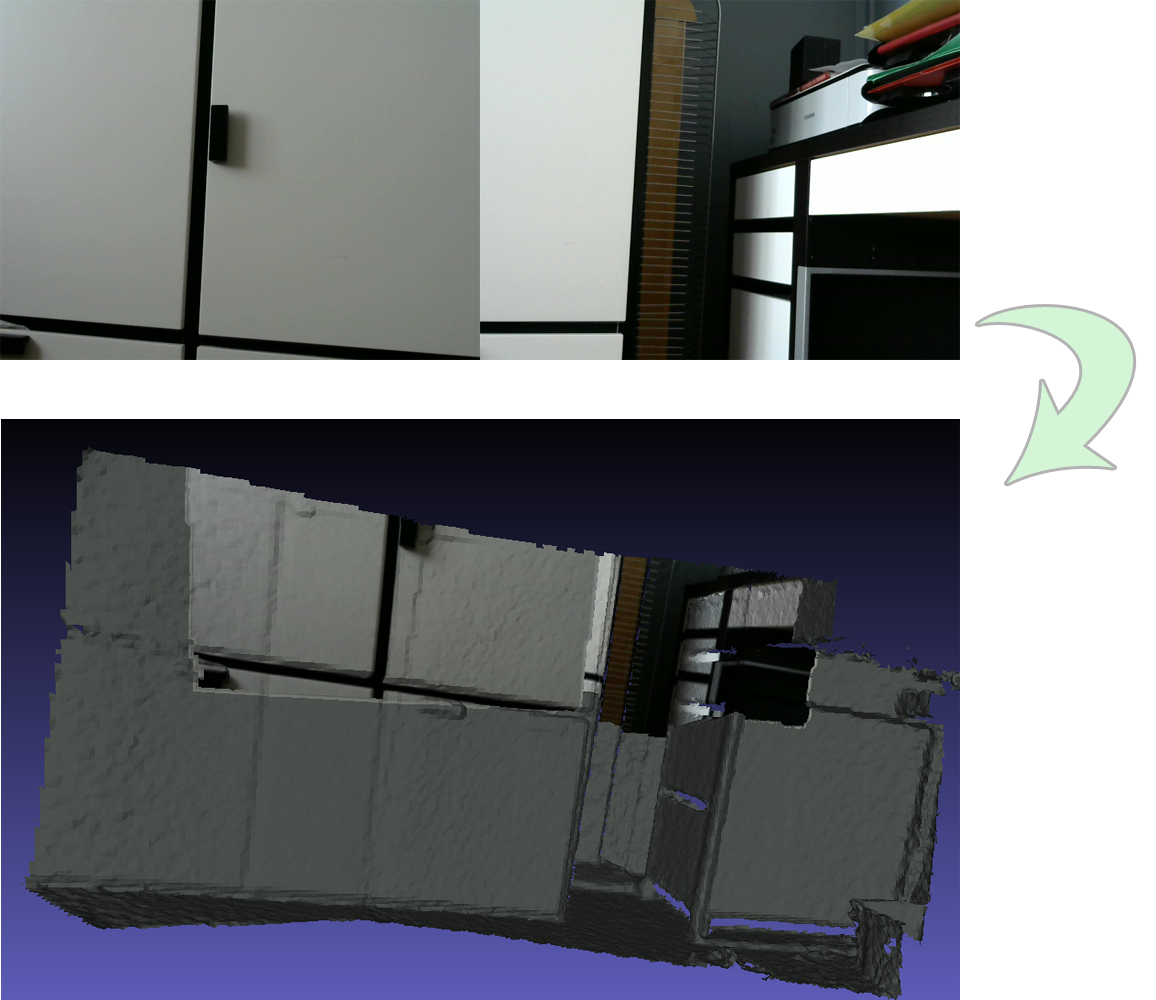
\includegraphics[width=1.0\textwidth]{images/result3.png}
\label{fig:result3}
\end{figure}

\begin{figure}
\caption{Result 4}
\centering
    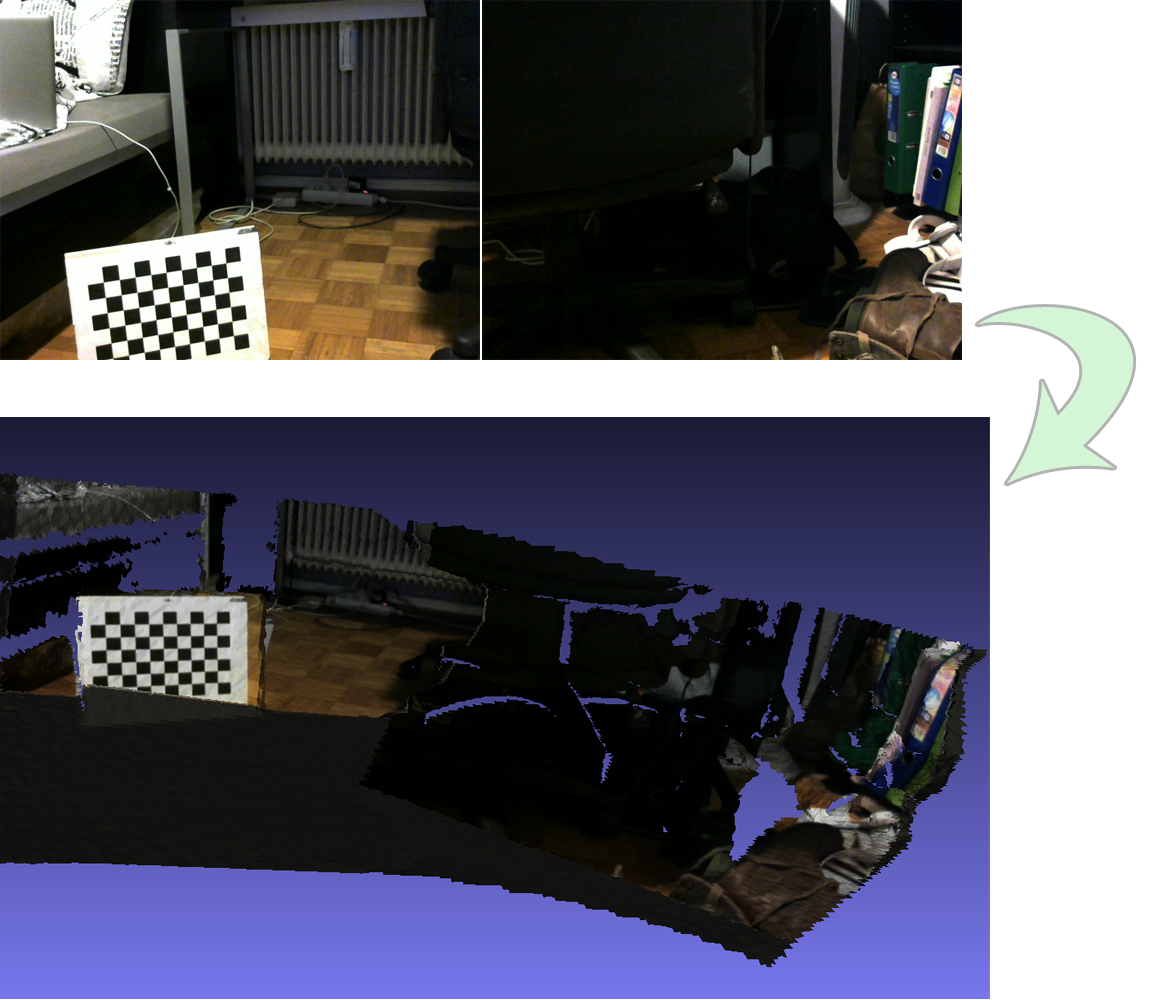
\includegraphics[width=1.0\textwidth]{images/result4.png}
\label{fig:result4}
\end{figure}

\section{Hamamatsu camera}
\label{sec:Hamamatsu camera}

For test purposes, so far only a webcam had been used as an external camera for this project. In real situations, a camera able to obtain IR information has to be utilized. The following paragraph describes such cameras and also discusses the potential issues that can arise when the Kinect is combined with another IR camera.\\

As seen in Section~\ref{sec: ICG Applications}, the use of indocyanine green (ICG) coupled with IR cameras is recent. One of the cameras of interest is the Photodynamic Eye (PDE) Hamamatsu camera (see Figure~\ref{fig:hamamatsu} \cite{pde}). Indeed, the PDE camera has already been used in several studies. \\

Unno et al. (2007) \cite{unno_quantitative_2008} employs it as a diagnostic imaging technique to assess lymph function. They injected 0.3 ml of ICG at the dorsum of the feet and observed the time required by the ICG to reach the groin area. Gotoh et al. (2009) \cite{gotoh_novel_2009} used the PDE camera to make the distinction between tumor and normal tissues. Rasmussen et al (2010) \cite{rasmussen_lymphatic_2009}. conducted a study on healthy patients to observe their lymphatic system architecture (see Figure~\ref{fig:hamaResults0}). More recently, Tagaya et al. (2010) \cite{tagaya_non-invasive_2010} utilized it to identify sentinel lymph nodes in patients with breast cancer. In all those studies, the PDE camera provided satisfactory images to produce good results.\\

\begin{figure}
\caption{Photodynamic (PDE) Hamamatsu camera}
\centering
    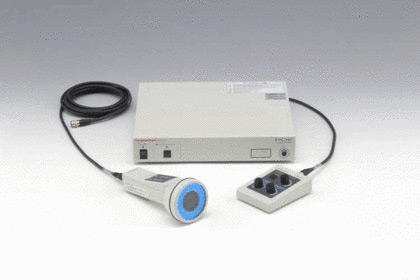
\includegraphics[width=0.7\textwidth]{images/hamamatsu.jpg}
\label{fig:hamamatsu}
\end{figure}

\begin{figure}
\caption{Images of healthy lymphatics typically seen in normal subjects}
\centering
    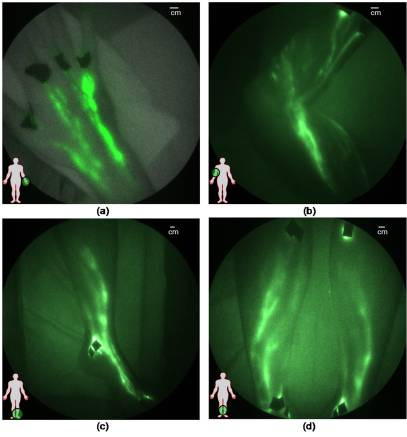
\includegraphics[width=0.7\textwidth]{images/imageICGLymph.png}
\label{fig:hamaResults0}
\end{figure}

The PDE camera uses the fluorescence principle described in section~\ref{sec:fluorescence principle}. The camera excites the ICG with an IR light at a wavelength of 760 nm \cite{tagaya_non-invasive_2010} and filters out light below 820 nm \cite{gotoh_novel_2009}. \\

Note that the ICG can be exited at a range between 760nm and 785nm and it emits light between 820 and 840 nm \cite{marshall_near-infrared_2010}. As said earlier, issues can arise with the Kinect camera since it also produces IR light. Figure~\ref{fig:kinectSpectrum} \cite{kolomenski_realization_2013} shows the spectral sensitivity of the Kinect as a function of the light wavelength. As it can be seen, lights at a wavelength of 760 nm (the wavelength used by the PDE Hamamatsu camera) does not affect much the Kinect therefore the PDE Hamamatsu camera will not affect the performances of the Kinect. However, the IR emitter from the Kinect produces IR dots at a wavelength of 830 nm \cite{kramer_introducing_2012} therefore those dots might be seen by the PDE hamamatsu camera. Indeed, some tests have been conducted using both the Kinect and the PDE camera, Figure~\ref{fig:PDEOK} shows a picture taken from the PDE camera when no Kinect was in used while Figure~\ref{fig:PDENotOK} shows the same area after that is has been targeted by a Kinect camera. As it can be seen, the IR light emitted by the Kinect greatly affects the measurements of the PDE camera. A possible solution would be to use some filters or to turn off the IR emitter of the Kinect when pictures are taken by the PDE camera. If the later is used, one should be careful that the Kinect does not reset its camera pose during the process otherwise the surface acquisition will be prone to errors. Future investigations should be carried out in order to solve this issue.\\
  
\begin{figure}
\caption{IR Kinect sensor spectrum}
\centering
    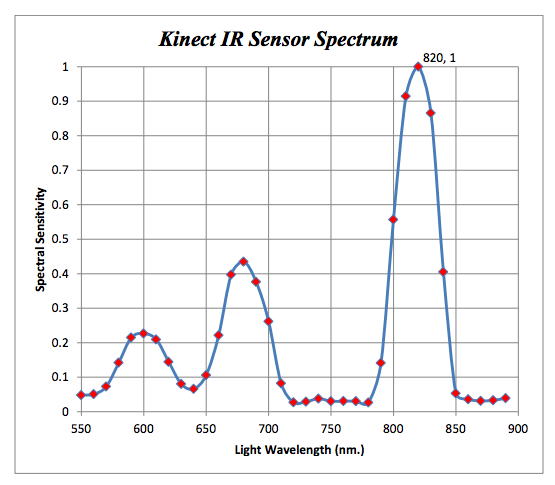
\includegraphics[width=1.0\textwidth]{images/kinectSpectrum.png}
\label{fig:kinectSpectrum}
\end{figure}

\begin{figure}
\caption{PDE Hamamatsu camera in used with no Kinect}
\centering
    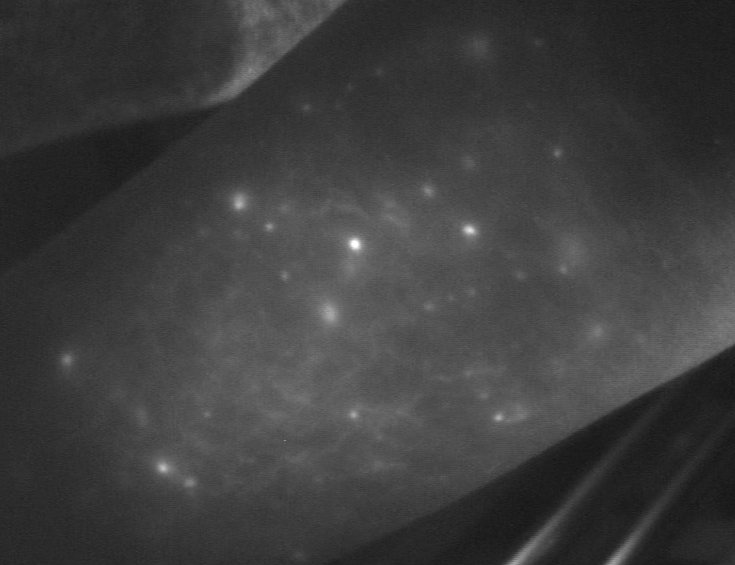
\includegraphics[width=0.7\textwidth]{images/PDEOK.png}
\label{fig:PDEOK}
\end{figure}

\begin{figure}
\caption{PDE Hamamatsu camera in used with a Kinect}
\centering
    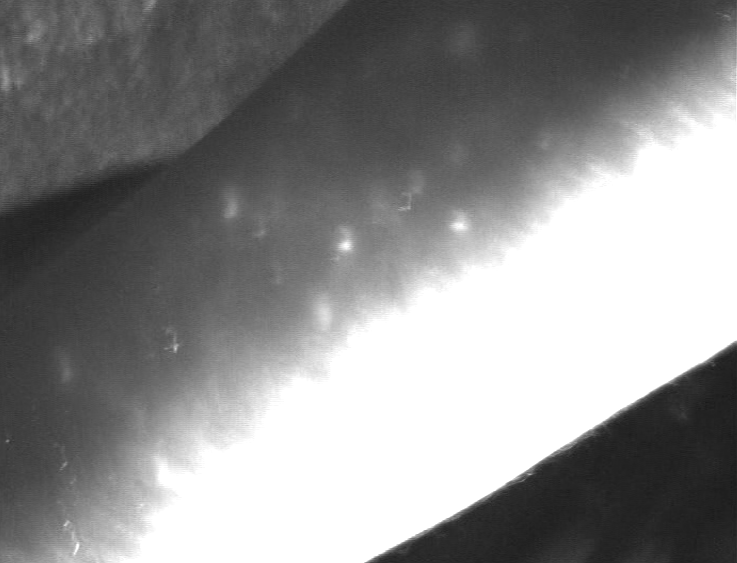
\includegraphics[width=0.7\textwidth]{images/PDENotOK.png}
\label{fig:PDENotOK}
\end{figure}

Note that other cameras exist, however studying them all is beyond the scope of this thesis, the interested reader can consult the article written by Marshall et al. (2012) \cite{marshall_near-infrared_2010} for a more exhaustive study of other cameras.


